% Options for packages loaded elsewhere
% Options for packages loaded elsewhere
\PassOptionsToPackage{unicode}{hyperref}
\PassOptionsToPackage{hyphens}{url}
%
\documentclass[
  11pt,
  ignorenonframetext,
  aspectratio=169,
]{beamer}
\newif\ifbibliography
\usepackage{pgfpages}
\setbeamertemplate{caption}[numbered]
\setbeamertemplate{caption label separator}{: }
\setbeamercolor{caption name}{fg=normal text.fg}
\beamertemplatenavigationsymbolsempty
% remove section numbering
\setbeamertemplate{part page}{
  \centering
  \begin{beamercolorbox}[sep=16pt,center]{part title}
    \usebeamerfont{part title}\insertpart\par
  \end{beamercolorbox}
}
\setbeamertemplate{section page}{
  \centering
  \begin{beamercolorbox}[sep=12pt,center]{section title}
    \usebeamerfont{section title}\insertsection\par
  \end{beamercolorbox}
}
\setbeamertemplate{subsection page}{
  \centering
  \begin{beamercolorbox}[sep=8pt,center]{subsection title}
    \usebeamerfont{subsection title}\insertsubsection\par
  \end{beamercolorbox}
}
% Prevent slide breaks in the middle of a paragraph
\widowpenalties 1 10000
\raggedbottom
\AtBeginPart{
  \frame{\partpage}
}
\AtBeginSection{
  \ifbibliography
  \else
    \frame{\sectionpage}
  \fi
}
\AtBeginSubsection{
  \frame{\subsectionpage}
}
\usepackage{iftex}
\ifPDFTeX
  \usepackage[T1]{fontenc}
  \usepackage[utf8]{inputenc}
  \usepackage{textcomp} % provide euro and other symbols
\else % if luatex or xetex
  \usepackage{unicode-math} % this also loads fontspec
  \defaultfontfeatures{Scale=MatchLowercase}
  \defaultfontfeatures[\rmfamily]{Ligatures=TeX,Scale=1}
\fi
\usepackage{lmodern}

\ifPDFTeX\else
  % xetex/luatex font selection
\fi
% Use upquote if available, for straight quotes in verbatim environments
\IfFileExists{upquote.sty}{\usepackage{upquote}}{}
\IfFileExists{microtype.sty}{% use microtype if available
  \usepackage[]{microtype}
  \UseMicrotypeSet[protrusion]{basicmath} % disable protrusion for tt fonts
}{}
\makeatletter
\@ifundefined{KOMAClassName}{% if non-KOMA class
  \IfFileExists{parskip.sty}{%
    \usepackage{parskip}
  }{% else
    \setlength{\parindent}{0pt}
    \setlength{\parskip}{6pt plus 2pt minus 1pt}}
}{% if KOMA class
  \KOMAoptions{parskip=half}}
\makeatother

\usepackage{color}
\usepackage{fancyvrb}
\newcommand{\VerbBar}{|}
\newcommand{\VERB}{\Verb[commandchars=\\\{\}]}
\DefineVerbatimEnvironment{Highlighting}{Verbatim}{commandchars=\\\{\}}
% Add ',fontsize=\small' for more characters per line
\usepackage{framed}
\definecolor{shadecolor}{RGB}{241,243,245}
\newenvironment{Shaded}{\begin{snugshade}}{\end{snugshade}}
\newcommand{\AlertTok}[1]{\textcolor[rgb]{0.68,0.00,0.00}{#1}}
\newcommand{\AnnotationTok}[1]{\textcolor[rgb]{0.37,0.37,0.37}{#1}}
\newcommand{\AttributeTok}[1]{\textcolor[rgb]{0.40,0.45,0.13}{#1}}
\newcommand{\BaseNTok}[1]{\textcolor[rgb]{0.68,0.00,0.00}{#1}}
\newcommand{\BuiltInTok}[1]{\textcolor[rgb]{0.00,0.23,0.31}{#1}}
\newcommand{\CharTok}[1]{\textcolor[rgb]{0.13,0.47,0.30}{#1}}
\newcommand{\CommentTok}[1]{\textcolor[rgb]{0.37,0.37,0.37}{#1}}
\newcommand{\CommentVarTok}[1]{\textcolor[rgb]{0.37,0.37,0.37}{\textit{#1}}}
\newcommand{\ConstantTok}[1]{\textcolor[rgb]{0.56,0.35,0.01}{#1}}
\newcommand{\ControlFlowTok}[1]{\textcolor[rgb]{0.00,0.23,0.31}{\textbf{#1}}}
\newcommand{\DataTypeTok}[1]{\textcolor[rgb]{0.68,0.00,0.00}{#1}}
\newcommand{\DecValTok}[1]{\textcolor[rgb]{0.68,0.00,0.00}{#1}}
\newcommand{\DocumentationTok}[1]{\textcolor[rgb]{0.37,0.37,0.37}{\textit{#1}}}
\newcommand{\ErrorTok}[1]{\textcolor[rgb]{0.68,0.00,0.00}{#1}}
\newcommand{\ExtensionTok}[1]{\textcolor[rgb]{0.00,0.23,0.31}{#1}}
\newcommand{\FloatTok}[1]{\textcolor[rgb]{0.68,0.00,0.00}{#1}}
\newcommand{\FunctionTok}[1]{\textcolor[rgb]{0.28,0.35,0.67}{#1}}
\newcommand{\ImportTok}[1]{\textcolor[rgb]{0.00,0.46,0.62}{#1}}
\newcommand{\InformationTok}[1]{\textcolor[rgb]{0.37,0.37,0.37}{#1}}
\newcommand{\KeywordTok}[1]{\textcolor[rgb]{0.00,0.23,0.31}{\textbf{#1}}}
\newcommand{\NormalTok}[1]{\textcolor[rgb]{0.00,0.23,0.31}{#1}}
\newcommand{\OperatorTok}[1]{\textcolor[rgb]{0.37,0.37,0.37}{#1}}
\newcommand{\OtherTok}[1]{\textcolor[rgb]{0.00,0.23,0.31}{#1}}
\newcommand{\PreprocessorTok}[1]{\textcolor[rgb]{0.68,0.00,0.00}{#1}}
\newcommand{\RegionMarkerTok}[1]{\textcolor[rgb]{0.00,0.23,0.31}{#1}}
\newcommand{\SpecialCharTok}[1]{\textcolor[rgb]{0.37,0.37,0.37}{#1}}
\newcommand{\SpecialStringTok}[1]{\textcolor[rgb]{0.13,0.47,0.30}{#1}}
\newcommand{\StringTok}[1]{\textcolor[rgb]{0.13,0.47,0.30}{#1}}
\newcommand{\VariableTok}[1]{\textcolor[rgb]{0.07,0.07,0.07}{#1}}
\newcommand{\VerbatimStringTok}[1]{\textcolor[rgb]{0.13,0.47,0.30}{#1}}
\newcommand{\WarningTok}[1]{\textcolor[rgb]{0.37,0.37,0.37}{\textit{#1}}}

\usepackage{longtable,booktabs,array}
\newcounter{none} % for unnumbered tables
\usepackage{calc} % for calculating minipage widths
\usepackage{caption}
% Make caption package work with longtable
\makeatletter
\def\fnum@table{\tablename~\thetable}
\makeatother
\usepackage{graphicx}
\makeatletter
\newsavebox\pandoc@box
\newcommand*\pandocbounded[1]{% scales image to fit in text height/width
  \sbox\pandoc@box{#1}%
  \Gscale@div\@tempa{\textheight}{\dimexpr\ht\pandoc@box+\dp\pandoc@box\relax}%
  \Gscale@div\@tempb{\linewidth}{\wd\pandoc@box}%
  \ifdim\@tempb\p@<\@tempa\p@\let\@tempa\@tempb\fi% select the smaller of both
  \ifdim\@tempa\p@<\p@\scalebox{\@tempa}{\usebox\pandoc@box}%
  \else\usebox{\pandoc@box}%
  \fi%
}
% Set default figure placement to htbp
\def\fps@figure{htbp}
\makeatother





\setlength{\emergencystretch}{3em} % prevent overfull lines

\providecommand{\tightlist}{%
  \setlength{\itemsep}{0pt}\setlength{\parskip}{0pt}}



 


\setbeamertemplate{navigation symbols}{}
\setbeamertemplate{footline}[frame number]
\setbeamertemplate{itemize items}[circle]
\setbeamertemplate{itemize subitem}[triangle]
\setbeamercolor{frametitle}{fg=black}
\setbeamerfont{frametitle}{series=\bfseries}
\usepackage{amsmath}
\newcommand{\indep}{\perp\!\!\!\perp}
\usepackage{booktabs}
\usepackage{array}
\usepackage{adjustbox}
\newcommand{\src}[1]{\par\vspace{-0.2em}{\tiny\color{gray} Source: #1}\par}
\usepackage{fancyvrb}
\fvset{fontsize=\scriptsize}
\makeatletter
\def\verbatim@font{\scriptsize\ttfamily}
\makeatother
\makeatletter
\@ifpackageloaded{caption}{}{\usepackage{caption}}
\AtBeginDocument{%
\ifdefined\contentsname
  \renewcommand*\contentsname{Table of contents}
\else
  \newcommand\contentsname{Table of contents}
\fi
\ifdefined\listfigurename
  \renewcommand*\listfigurename{List of Figures}
\else
  \newcommand\listfigurename{List of Figures}
\fi
\ifdefined\listtablename
  \renewcommand*\listtablename{List of Tables}
\else
  \newcommand\listtablename{List of Tables}
\fi
\ifdefined\figurename
  \renewcommand*\figurename{Figure}
\else
  \newcommand\figurename{Figure}
\fi
\ifdefined\tablename
  \renewcommand*\tablename{Table}
\else
  \newcommand\tablename{Table}
\fi
}
\@ifpackageloaded{float}{}{\usepackage{float}}
\floatstyle{ruled}
\@ifundefined{c@chapter}{\newfloat{codelisting}{h}{lop}}{\newfloat{codelisting}{h}{lop}[chapter]}
\floatname{codelisting}{Listing}
\newcommand*\listoflistings{\listof{codelisting}{List of Listings}}
\makeatother
\makeatletter
\makeatother
\makeatletter
\@ifpackageloaded{caption}{}{\usepackage{caption}}
\@ifpackageloaded{subcaption}{}{\usepackage{subcaption}}
\makeatother

\usepackage{bookmark}
\IfFileExists{xurl.sty}{\usepackage{xurl}}{} % add URL line breaks if available
\urlstyle{same}
\hypersetup{
  pdftitle={Difference-in-Differences: Staggered Adoption},
  pdfauthor={Professor Ji-Woong Chung},
  hidelinks,
  pdfcreator={LaTeX via pandoc}}


\title{\texorpdfstring{Difference-in-Differences: Staggered
Adoption}{Difference-in-Differences: Staggered Adoption}}
\subtitle{\texorpdfstring{BUSS975: Causal Inference in Financial
Research}{BUSS975: Causal Inference in Financial Research}}
\author{Professor Ji-Woong Chung}
\date{}
\institute{Korea University}

\begin{document}
\frame{\titlepage}


\begin{frame}{Where we left off}
\protect\phantomsection\label{where-we-left-off}
\begin{itemize}
\tightlist
\item
  Lecture 7b: under staggered adoption, TWFE is a weighted average of
  \textbf{every} \(2 \times 2\) in the data, weighted by group size and
  treatment variance.
\item
  Some of those \(2 \times 2\)'s use an \textbf{already-treated}
  control. They subtract the control's own growing effect: \[
  \operatorname{plim}\hat\delta^{TWFE} = \text{VWATT} + \text{VWPT} - \Delta\text{ATT}.
  \]
\item
  Baker simulation: all effects positive, parallel trends exact. True
  simple ATT \(82\); TWFE \(-6.69\). Weight \(0.50\) on forbidden
  comparisons averaging \(-65.2\).
\end{itemize}

\vspace{0.4em}

\begin{itemize}
\tightlist
\item
  Today: estimators that \textbf{never} make the forbidden comparison,
  how to read their event studies, and a checklist for your own design.
\end{itemize}
\end{frame}

\begin{frame}{The plan}
\protect\phantomsection\label{the-plan}
\begin{enumerate}
\tightlist
\item
  \textbf{Callaway and Sant'Anna}: build group-time \(2 \times 2\)'s,
  then aggregate.
\item
  \textbf{Sun and Abraham}: what goes wrong in the TWFE \emph{event
  study}, and the interaction-weighted fix.
\item
  \textbf{de Chaisemartin and D'Haultfoeuille}: treatments that switch
  off.
\item
  \textbf{Borusyak, Jaravel and Spiess}: imputation.
\item
  \textbf{Reading an event study}: long differences, short gaps, honest
  bounds.
\item
  \textbf{A checklist}, worked through Brazil's mental-health reform.
\end{enumerate}

\vspace{0.4em}

\begin{itemize}
\tightlist
\item
  One running question: \textbf{which \(2 \times 2\)'s are inside my
  estimate, and what weight does each carry?}
\end{itemize}
\end{frame}

\section{1. Callaway and Sant'Anna}\label{callaway-and-santanna}

\begin{frame}{Stop asking for one number}
\protect\phantomsection\label{stop-asking-for-one-number}
\begin{itemize}
\tightlist
\item
  TWFE asks for \textbf{one} \(\delta\) and lets OLS decide how to
  average. CS reverses the order:

  \begin{enumerate}
  \tightlist
  \item
    estimate many small, clean effects;
  \item
    average them with weights \textbf{you} choose.
  \end{enumerate}
\item
  The small effect is the \textbf{group-time ATT} (Callaway and
  Sant'Anna 2021). For the cohort first treated at \(g\), in calendar
  period \(t\), \[
  \text{ATT}(g, t) = \mathbb{E}[Y^1_t - Y^0_t \mid G_g = 1].
  \]
\item
  Example: \(\text{ATT}(1992, 1995)\) is the effect on firms treated in
  1992, measured in 1995, their fourth treated year.
\item
  Useful when effects depend on adoption date, change with time since
  treatment, or vary with macro conditions.
\end{itemize}
\end{frame}

\begin{frame}{Each \(\text{ATT}(g,t)\) is a \(2 \times 2\) you would
choose by hand}
\protect\phantomsection\label{each-textattgt-is-a-2-times-2-you-would-choose-by-hand}
Cohort \(g\) from its baseline \(g - 1\) to \(t\), against units
\textbf{untreated in both periods}. For \(\text{ATT}(1992, 1995)\) in
the Baker data:

\begin{center}\small
\begin{tabular}{lccl}
\toprule
Cohort & 1991 (baseline) & 1995 & Role \\
\midrule
1986 & treated & treated & already treated: \textbf{excluded} \\
1992 & untreated & treated & the treated group \\
1998 & untreated & untreated & control (not yet treated) \\
2004 & untreated & untreated & control (not yet treated) \\
\bottomrule
\end{tabular}
\end{center}

\begin{itemize}
\tightlist
\item
  \(\widehat{\text{ATT}}(1992, 1995) = 32.02\); the truth is
  \(8 \times 4 = 32\).
\item
  Controls are either \textbf{never-treated} or
  \textbf{not-yet-treated}. Never a unit that is already treated.
\end{itemize}
\end{frame}

\begin{frame}{With covariates, and the assumptions}
\protect\phantomsection\label{with-covariates-and-the-assumptions}
The \(2 \times 2\) becomes 7b's IPW, OR or DR estimator, with a score
estimated among cohort \(g\) and its controls \(C\),
\(\hat p(X) = \Pr(G_g = 1 \mid X, G_g + C = 1)\): \[
\text{ATT}(g,t) = \mathbb{E}\!\left[\left(\frac{G_g}{\mathbb{E}[G_g]} - \frac{\frac{\hat p(X) C}{1 - \hat p(X)}}{\mathbb{E}\!\left[\frac{\hat p(X) C}{1 - \hat p(X)}\right]}\right)\big(Y_t - Y_{g-1}\big)\right].
\]

\begin{enumerate}
\tightlist
\item
  \textbf{Absorbing} treatment: once on, always on.
\item
  \textbf{No anticipation.}
\item
  \textbf{Parallel trends}, given \(X\), between cohort \(g\) and the
  chosen controls.
\item
  \textbf{Weak overlap}, and one correct nuisance model if \(X\) is
  used.
\end{enumerate}

The score changes cohort by cohort, because the pool of untreated
controls shrinks.
\end{frame}

\begin{frame}{Aggregation: the weights are yours}
\protect\phantomsection\label{aggregation-the-weights-are-yours}
Once you have the cells, any non-negative average of them is a valid
parameter:

\begin{center}\small
\begin{tabular}{lll}
\toprule
Parameter & Averages $\text{ATT}(g,t)$ over & Answers \\
\midrule
Simple ATT & all post-treatment cells, by size & average effect on treated unit-years \\
Group ATT & $t \ge g$ within cohort, then cohorts & average effect per adopting cohort \\
Event study $\theta(\ell)$ & cohorts at the same $\ell = t - g$ & how effects evolve with exposure \\
Calendar $\theta(t)$ & cohorts treated by $t$ & effect in a given year \\
\bottomrule
\end{tabular}
\end{center}

\begin{itemize}
\tightlist
\item
  Compare TWFE: one average, weights set by treatment variance, some
  cells from forbidden comparisons.
\item
  Here the weights are written down \textbf{before} estimation and have
  a meaning.
\end{itemize}
\end{frame}

\begin{frame}{Which cells exist}
\protect\phantomsection\label{which-cells-exist}
Baker data, dynamic effects. A cell is estimable only while some unit is
still untreated at \(t\):

\begin{center}\scriptsize
\begin{tabular}{lccccc}
\toprule
Year & $g = 1986$ & $g = 1992$ & $g = 1998$ & $g = 2004$ & Untreated control? \\
\midrule
1985 & 0 & 0 & 0 & 0 & yes \\
1986 & 10 & 0 & 0 & 0 & yes \\
1992 & 70 & 8 & 0 & 0 & yes \\
1998 & 130 & 56 & 6 & 0 & yes \\
2003 & 180 & 96 & 36 & 0 & yes \\
2004 & 190 & 104 & 42 & 4 & \textbf{no} \\
2009 & 240 & 144 & 72 & 24 & \textbf{no} \\
\midrule
ATT($g$), all cells & 125 & 76 & 39 & 14 & \\
ATT($g$), feasible cells & 95 & 52 & 21 & -- & \\
\bottomrule
\end{tabular}
\end{center}

\begin{itemize}
\tightlist
\item
  From 2004 everyone is treated. The 2004 cohort exists only as a
  control.
\end{itemize}
\end{frame}

\begin{frame}{What the data can and cannot tell you}
\protect\phantomsection\label{what-the-data-can-and-cannot-tell-you}
\begin{itemize}
\tightlist
\item
  Feasible simple ATT \(68.3\) and feasible group ATT \(56\), against
  \(82\) and \(63.5\) using every cell.
\item
  The gap is not estimator bias. The late, large effects are not
  identified by \textbf{any} honest comparison: there is no one left to
  compare with.
\item
  TWFE used those years anyway, through forbidden comparisons. That is
  where its answer came from.
\end{itemize}

\vspace{0.4em}

\begin{itemize}
\tightlist
\item
  A general lesson: an honest estimator may target a \textbf{smaller}
  parameter than you hoped. Say which one.
\end{itemize}
\end{frame}

\begin{frame}{One cell by hand, then all of them}
\protect\phantomsection\label{one-cell-by-hand-then-all-of-them}
\(\text{ATT}(1986, 1986)\): the 1986 cohort's change from 1985 to 1986,
less the change for firms not yet treated in 1986 (the 1992, 1998 and
2004 cohorts): \[
\widehat{\text{ATT}}(1986,1986) = (\bar y_{1986}^{\,g=1986} - \bar y_{1985}^{\,g=1986}) - (\bar y_{1986}^{\,C} - \bar y_{1985}^{\,C}) = 10.03 \qquad (\text{truth } 10).
\]

\begin{itemize}
\tightlist
\item
  Four averages and three subtractions. With covariates they become four
  \emph{weighted} averages.
\item
  That is the whole estimator; the package only loops over \((g, t)\).
\end{itemize}
\end{frame}

\begin{frame}[fragile]{All \(36\) feasible cells, aggregated}
\protect\phantomsection\label{all-36-feasible-cells-aggregated}
\begin{center}\small
\begin{tabular}{lccc}
\toprule
 & Estimate & Feasible truth & Full truth \\
\midrule
Simple ATT: mean over cells & $68.34$ & $68.33$ & $82$ \\
Group ATT: mean of ATT($g$) & $56.00$ & $56$ & $63.5$ \\
\bottomrule
\end{tabular}
\end{center}

\begin{itemize}
\tightlist
\item
  ATT(\(g\)) by cohort: \(95.0\), \(52.0\), \(21.0\), against \(95\),
  \(52\), \(21\).
\item
  TWFE said \(-6.69\). Same data, same assumptions; the only change is
  which comparisons are allowed.
\item
  Stata:
  \texttt{csdid2\ y,\ ivar(id)\ time(year)\ gvar(treat\_date)\ notyet\ method(stdipw)\ long2}.
  R: \texttt{did::att\_gt}.
\end{itemize}
\end{frame}

\begin{frame}{Event studies from building blocks}
\protect\phantomsection\label{event-studies-from-building-blocks}
\begin{center}
\includegraphics[width=0.76\linewidth,height=\textheight,keepaspectratio]{07c_did_staggered_files/figure-beamer/baker-es-1.pdf}
\end{center}

\begin{itemize}
\tightlist
\item
  Average the cells by \textbf{relative time} \(\ell = t - g\). Years to
  2003, so the 2004 cohort is the untreated control.
\end{itemize}
\end{frame}

\begin{frame}{Reading the event study: CS and SA}
\protect\phantomsection\label{reading-the-event-study-cs-and-sa}
\begin{itemize}
\tightlist
\item
  CS and SA sit on the truth.

  \begin{itemize}
  \tightlist
  \item
    At \(\ell = 0\) all three cohorts contribute:
    \((10 + 8 + 6)/3 = 8\).
  \item
    At \(\ell = 6\) only 1986 and 1992 remain: \((70 + 56)/2 = 63\).
  \end{itemize}
\item
  The staircase is real, but partly a \textbf{composition effect}: later
  lags are early adopters' effects.
\item
  Moving right along the axis changes both the time since treatment and
  \textbf{who is averaged}.
\end{itemize}
\end{frame}

\begin{frame}{Reading the event study: what went wrong with TWFE}
\protect\phantomsection\label{reading-the-event-study-what-went-wrong-with-twfe}
\begin{itemize}
\tightlist
\item
  The TWFE line, as usually run, gives the 2004 cohort lead dummies too.
  No unit is left as a reference.
\item
  Relative time is then collinear with the fixed effects, and fixest
  \textbf{silently drops \(\ell = 12, \dots, 17\)}.
\item
  Those dropped post periods load onto every other coefficient (Section
  2): a falling ``pre-trend'' and near-zero effects that do not exist.
\end{itemize}

\vspace{0.4em}

\begin{itemize}
\tightlist
\item
  Code the 2004 cohort as never treated and TWFE is identified: leads
  \(2.0\) to \(0.4\), \(\hat\mu_0 = 9.0\), \(\hat\mu_{6} = 61.5\),
  against \(8\) and \(63\).
\item
  Contaminated, but mildly. Most of the damage in the figure came from
  the dropped periods.
\end{itemize}
\end{frame}

\begin{frame}{Castle doctrine, all cohorts: CS against TWFE}
\protect\phantomsection\label{castle-doctrine-all-cohorts-cs-against-twfe}
\begin{center}\small
\begin{tabular}{lcccccccc}
\toprule
 & Static & $\ell=-3$ & $\ell=-2$ & $\ell=0$ & $\ell=1$ & $\ell=2$ & $\ell=3$ & $\ell=4$ \\
\midrule
TWFE & $0.082$ & $0.054$ & $0.059$ & $0.092$ & $0.106$ & $0.115$ & $0.110$ & $0.084$ \\
CS, never-treated & $0.110$ & $0.057$ & $0.058$ & $0.097$ & $0.112$ & $0.112$ & $0.137$ & $0.093$ \\
\bottomrule
\end{tabular}
\end{center}

\begin{itemize}
\tightlist
\item
  CS: \(20\) group-time cells against the \(29\) never-adopting states,
  weighted by cohort size (\(1, 13, 4, 2, 1\) states). Each cell uses
  the fixed baseline \(g-1\).
\end{itemize}
\end{frame}

\begin{frame}{Castle doctrine: why the static numbers differ}
\protect\phantomsection\label{castle-doctrine-why-the-static-numbers-differ}
\begin{itemize}
\tightlist
\item
  Static CS: \(11\) percent. TWFE: \(8\) percent.
\item
  Not the forbidden comparisons: TWFE's clean treated-vs-never
  \(2 \times 2\)'s alone average \(0.088\).
\item
  The rest is \textbf{weighting and baseline}:

  \begin{itemize}
  \tightlist
  \item
    TWFE weights cohorts by treatment variance and compares \emph{all}
    post years with \emph{all} pre years;
  \item
    CS weights by cohort size and differences each year from \(g - 1\).
  \end{itemize}
\item
  The event-study coefficients barely move. Here the two agree on the
  story.
\item
  In Baker, Larcker and Wang's replications they did not. You cannot
  know which case you are in without looking.
\end{itemize}
\end{frame}

\section{2. Sun and Abraham}\label{sun-and-abraham}

\begin{frame}{The TWFE event study and its three assumptions}
\protect\phantomsection\label{the-twfe-event-study-and-its-three-assumptions}
The canonical event study under differential timing: \[
Y_{it} = \alpha_i + \lambda_t + \sum_{\ell \ne -1}\mu_\ell\,\mathbf{1}\{t - E_i = \ell\} + \varepsilon_{it}.
\]

For \(\hat\mu_\ell\) to mean ``the effect \(\ell\) periods after
treatment'', three things must hold:

\begin{enumerate}
\tightlist
\item
  \textbf{parallel trends} for every cohort;
\item
  \textbf{no anticipation};
\item
  a \textbf{homogeneous effect profile}: every cohort follows the same
  path of effects after treatment.
\end{enumerate}

\begin{itemize}
\tightlist
\item
  Dynamics are fine. What is not fine is cohorts with \textbf{different}
  dynamics: early adopters' effects growing faster, say.
\end{itemize}
\end{frame}

\begin{frame}{Contamination: what each coefficient really contains}
\protect\phantomsection\label{contamination-what-each-coefficient-really-contains}
Sun and Abraham (2021) write each \(\hat\mu_\ell\) in terms of
cohort-specific effects \(\text{CATT}_{e,\ell}\):

\[
\hat\mu_\ell = \underbrace{\sum_e w^{\ell}_{e,\ell}\,\text{CATT}_{e,\ell}}_{\text{own period: sum to } 1} +
\underbrace{\sum_{\ell' \ne \ell}\sum_e w^{\ell}_{e,\ell'}\,\text{CATT}_{e,\ell'}}_{\text{other included periods: sum to } 0} +
\underbrace{\sum_{\ell' \in \text{excl}}\sum_e w^{\ell}_{e,\ell'}\,\text{CATT}_{e,\ell'}}_{\text{excluded periods: sum to } -1}.
\]

\begin{itemize}
\tightlist
\item
  Weights that sum to zero must contain negatives: the coefficient for
  \(\ell = -2\) can contain effects from \(\ell = +5\).
\item
  \textbf{Contamination}, the same disease as judge dummies in Lecture
  5b (Goldsmith-Pinkham, Hull and Kolesár 2024).
\end{itemize}
\end{frame}

\begin{frame}{The two-cohort example}
\protect\phantomsection\label{the-two-cohort-example}
Three periods (\(t = 0, 1, 2\)). Cohort 1 is treated in period 1, cohort
2 in period 2. Include dummies for \(\ell \in \{-2, 0\}\); exclude
\(\{-1, +1\}\). Then \[
\hat\mu_{-2} = \underbrace{\text{CATT}_{2,-2}}_{\text{own}} + \underbrace{\tfrac12\text{CATT}_{1,0} - \tfrac12\text{CATT}_{2,0}}_{\text{other included}} + \underbrace{\tfrac12\text{CATT}_{1,1} - \text{CATT}_{1,-1} - \tfrac12\text{CATT}_{2,-1}}_{\text{excluded}}.
\]

\begin{itemize}
\tightlist
\item
  A \textbf{pre-period} coefficient, built from five cohort-period
  effects, some of them \textbf{post-treatment}.
\item
  Now switch on the three assumptions one at a time.
\end{itemize}
\end{frame}

\begin{frame}{Switching on the assumptions}
\protect\phantomsection\label{switching-on-the-assumptions}
\begin{itemize}
\tightlist
\item
  \textbf{Parallel trends} makes every term a causal effect rather than
  a trend difference.
\item
  \textbf{No anticipation} deletes the three pre-period terms.
\item
  \textbf{Homogeneous profiles} make
  \(\text{CATT}_{1,0} = \text{CATT}_{2,0}\), so the middle cancels.
\end{itemize}

\vspace{0.4em}

\begin{itemize}
\tightlist
\item
  What survives is \(\tfrac12\text{CATT}_{1,1}\): a ``pre-trend'' made
  of a \textbf{post-treatment effect from an excluded period}.
\item
  Nobody excludes a post period on purpose. Software does it when no
  unit is untreated: fixest dropped \(\ell \ge 12\) in the Baker figure.
  Binning distant lags into the reference group does it too.
\item
  With heterogeneous profiles the middle term survives as well.
\end{itemize}
\end{frame}

\begin{frame}[fragile]{The interaction-weighted estimator}
\protect\phantomsection\label{the-interaction-weighted-estimator}
\begin{enumerate}
\tightlist
\item
  Run a \(2 \times 2\) for \textbf{each cohort and each relative
  period}, against the \textbf{never-treated} or the
  \textbf{last-treated} cohort. These are the \(\text{CATT}_{e,\ell}\).
\item
  Weight each cohort by its share of the units observed at relative time
  \(\ell\).
\item
  Sum. The result is consistent for \(\text{ATT}_\ell\) under parallel
  trends and no anticipation alone.
\end{enumerate}

\vspace{0.3em}

\begin{itemize}
\tightlist
\item
  In the Baker figure it gives the truth, with the 2004 cohort as
  control. R: \texttt{fixest::sunab(cohort,\ period)}; Stata:
  \texttt{eventstudyinteract}.
\item
  The key difference from CS is the control: \textbf{not} the
  not-yet-treated.
\item
  CS and SA are the same building blocks with different default controls
  and aggregations. If they disagree, parallel trends holds for one
  control group and not the other: a fact about your design.
\end{itemize}
\end{frame}

\section{3. de Chaisemartin and
D'Haultfoeuille}\label{de-chaisemartin-and-dhaultfoeuille}

\begin{frame}[fragile]{Negative weights on unit-time effects}
\protect\phantomsection\label{negative-weights-on-unit-time-effects}
\begin{itemize}
\tightlist
\item
  dCDH diagnose the same disease one level down. TWFE is a weighted sum
  of \textbf{every treated cell's effect}, and some weights are
  \textbf{negative}.
\item
  Which cells? Mostly long-treated units in heavily treated periods:
  exactly the already-treated controls of 7b.
\item
  A negative weight means a \emph{larger} effect in that cell
  \emph{lowers} the coefficient.
\item
  If you must report TWFE, report the share of negative weights (Stata:
  \texttt{twowayfeweights}).
\item
  Bacon's weights are all positive and dCDH's are not. Both are right:
  Bacon weights \(2 \times 2\) \emph{comparisons}; dCDH weight
  \emph{treatment effects}.
\end{itemize}
\end{frame}

\begin{frame}[fragile]{Treatments that switch off: \(\text{DID}_M\)}
\protect\phantomsection\label{treatments-that-switch-off-textdid_m}
At each date, average two kinds of \(2 \times 2\):

\begin{itemize}
\tightlist
\item
  \textbf{joiners}: units switching \textbf{into} treatment at \(t\),
  against units untreated at both \(t-1\) and \(t\);
\item
  \textbf{leavers}: units switching \textbf{out}, against units treated
  at both.
\end{itemize}

\vspace{0.3em}

\begin{itemize}
\tightlist
\item
  So the treatment may \textbf{turn off}. With absorbing treatment it
  reduces to a joiner average.
\item
  The price is \textbf{no carryover}: the outcome at \(t\) depends on
  treatment at \(t\) only. The road is dry the moment it stops raining.
  That is no anticipation pointed the other way, and often harder to
  believe.
\item
  Newer work relaxes it: \texttt{did\_multiplegt\_dyn} lets outcomes
  depend on treatment history, and handles non-binary and continuous
  treatments.
\end{itemize}
\end{frame}

\section{4. Imputation}\label{imputation}

\begin{frame}{Borusyak, Jaravel and Spiess (2024)}
\protect\phantomsection\label{borusyak-jaravel-and-spiess-2024}
\begin{enumerate}
\tightlist
\item
  Using \textbf{untreated cells only} (never-treated and
  not-yet-treated), fit
  \(Y_{it} = \alpha_i + \tau_t + \varepsilon_{it}\).
\item
  Predict \(\hat Y^0_{it} = \hat\alpha_i + \hat\tau_t\) for every
  treated cell.
\item
  \(\hat\tau_{it} = Y_{it} - \hat Y^0_{it}\) for each treated cell;
  average with the weights your target parameter demands.
\item
  Standard errors from the implied linear combination of outcomes.
\end{enumerate}

\vspace{0.4em}

\begin{itemize}
\tightlist
\item
  Intuition: the unit effect \(\hat\alpha_i\) comes from the unit's own
  pre-treatment years; the year effect \(\hat\tau_t\) comes from whoever
  is untreated that year.
\item
  Treated cells never help estimate the counterfactual, so no treated
  unit can act as a control.
\end{itemize}
\end{frame}

\begin{frame}{Imputation on the Baker data, by hand}
\protect\phantomsection\label{imputation-on-the-baker-data-by-hand}
\begin{itemize}
\tightlist
\item
  Years to 2003; after that no one is untreated, so there is no year
  effect to estimate.
\item
  Simple ATT \(68.33\) against CS's \(68.34\). Cohort ATTs \(95.0\),
  \(52.0\), \(21.0\).
\end{itemize}

\vspace{0.4em}

\begin{itemize}
\tightlist
\item
  The assumption is stronger: parallel trends \textbf{in every period
  and for every unit}, not just from \(g - 1\).
\item
  In exchange it uses every pre-period, and it is the most efficient
  under homoskedasticity.
\item
  Wooldridge (2021) is numerically the same in balanced panels; Gardner
  (2021) is the two-stage version.
\end{itemize}
\end{frame}

\begin{frame}{Four estimators side by side}
\protect\phantomsection\label{four-estimators-side-by-side}
\begin{center}\scriptsize
\begin{tabular}{lllll}
\toprule
 & Controls & Baseline & Parallel trends needed & Treatment \\
\midrule
CS & never or not-yet-treated & $g - 1$ & from $g - 1$ to $t$ & absorbing \\
SA & never or last-treated & $\ell = -1$ & cohort vs. that control & absorbing \\
dCDH & same status at $t-1$ and $t$ & $t - 1$ & one period at a time & can switch; no carryover \\
BJS & all untreated cells & all pre-periods & every period, every unit & absorbing \\
\bottomrule
\end{tabular}
\end{center}

\begin{itemize}
\tightlist
\item
  All four refuse the forbidden comparison. They differ in
  \textbf{which} clean comparison they trust.
\item
  Choose by the assumption, not the standard error: CS relies less on
  parallel trends far from the baseline; BJS buys precision with more of
  it.
\item
  Many covariates? Imputation or Wooldridge's regression may beat CS,
  whose propensity scores can run into support problems; the price is
  functional form.
\end{itemize}
\end{frame}

\begin{frame}{Does it matter? Finance and accounting}
\protect\phantomsection\label{does-it-matter-finance-and-accounting}
\begin{itemize}
\tightlist
\item
  Baker, Larcker and Wang (2022): over \(700\) DiD papers in top finance
  and accounting journals, about \(400\) with staggered adoption, nearly
  all estimated by TWFE.
\item
  They replicated two: \textbf{bank deregulation} (interstate branching)
  and \textbf{board reforms} across countries. With the estimators
  above, the headline results were weakened or overturned.
\item
  The mechanism is Baker's: effects that build over time, cohorts that
  differ, a regression that subtracts early adopters' growing effects
  from late adopters' estimates.
\end{itemize}
\end{frame}

\begin{frame}{What this means for your own paper}
\protect\phantomsection\label{what-this-means-for-your-own-paper}
\begin{itemize}
\tightlist
\item
  What Baker, Larcker and Wang do \textbf{not} say: that staggered DiD
  is dead, or every old result wrong.
\item
  What they do say: for a decade the field reported a number without
  knowing which comparisons were inside it.
\end{itemize}

\vspace{0.4em}

In a staggered design, report:

\begin{enumerate}
\tightlist
\item
  which \((g, t)\) cells are estimable;
\item
  which control group you use, and why;
\item
  how you aggregate, and what parameter that gives;
\item
  if you also report TWFE, the Bacon weights beside it.
\end{enumerate}
\end{frame}

\section{5. Reading an Event Study}\label{reading-an-event-study}

\begin{frame}{Two ways to compute a pre-period coefficient (Roth 2024)}
\protect\phantomsection\label{two-ways-to-compute-a-pre-period-coefficient-roth-2024}
\textbf{Long difference}: every period against \textbf{one} baseline,
\(\ell = -1\). This is what OLS does. \[
\hat\delta_{-3} = (\bar Y_T^{\,-3} - \bar Y_T^{\,-1}) - (\bar Y_C^{\,-3} - \bar Y_C^{\,-1}).
\] \textbf{Short gap}: every period against \textbf{the one before it}.
Some packages do this by default. \[
\hat\delta_{-3} = (\bar Y_T^{\,-3} - \bar Y_T^{\,-2}) - (\bar Y_C^{\,-3} - \bar Y_C^{\,-2}).
\]

\begin{itemize}
\tightlist
\item
  Both are four averages and three subtractions. They answer
  \textbf{different questions}: ``how far from the baseline?'' against
  ``how much did the gap change this year?''
\end{itemize}
\end{frame}

\begin{frame}{The same data, both ways}
\protect\phantomsection\label{the-same-data-both-ways}
\begin{center}\small
\begin{tabular}{lrrrrrrrrrrr}
\toprule
$\ell$ & $-5$ & $-4$ & $-3$ & $-2$ & $-1$ & $0$ & $1$ & $2$ & $3$ & $4$ & $5$ \\
\midrule
Long difference & -1.2 & -0.9 & -0.6 & -0.3 & 0.0 & 3.3 & 3.6 & 3.9 & 4.2 & 4.5 & 4.8 \\
Short gap & -- & 0.3 & 0.3 & 0.3 & 0.3 & 3.3 & 0.3 & 0.3 & 0.3 & 0.3 & 0.3 \\
\bottomrule
\end{tabular}
\end{center}

\begin{itemize}
\tightlist
\item
  Noise-free: the treated group trends \(0.3\) a year faster than
  controls throughout, plus an effect of \(3\) at \(\ell = 0\).
\item
  \textbf{Long:} pre-period coefficients slope up to zero, then keep
  climbing. The trend is visible.
\item
  \textbf{Short:} a flat \(0.3\) with one spike. The trend looks like a
  small constant, easy to read as ``no pre-trend''.
\item
  The tell: a coefficient \textbf{with a confidence interval} at
  \(\ell = -1\) means short gaps.
\end{itemize}
\end{frame}

\begin{frame}{Roth's picture: one dataset, three ways to plot it}
\protect\phantomsection\label{roths-picture-one-dataset-three-ways-to-plot-it}
\begin{center}
\includegraphics[width=1\linewidth,height=\textheight,keepaspectratio]{07c_did_staggered_files/figure-beamer/roth-panels-1.pdf}
\end{center}

\src{Simulated, after Roth (2024) and Cunningham (2025), Figure 10.12: one treated and one control group; the treated group trends $0.5$ a period faster, and the true effect is zero.}
\end{frame}

\begin{frame}{Reading Roth's picture}
\protect\phantomsection\label{reading-roths-picture}
\begin{itemize}
\tightlist
\item
  \textbf{(a) TWFE}: long differences. The pre-trend is a straight line
  through the baseline, and it carries on after treatment: the
  ``effects'' are the trend.
\item
  \textbf{(b) CS} and \textbf{dCDH}, as plotted by default: short gaps
  before treatment. The same trend becomes a flat row of small bumps at
  \(0.5\). Post-treatment coefficients are the same as TWFE's.
\item
  \textbf{(c) BJS}: pre-coefficients rise, then the series
  \textbf{kinks} at treatment.

  \begin{itemize}
  \tightlist
  \item
    The post estimates assume parallel trends in \textbf{all} periods;
    the pre estimates test it.
  \item
    If the trends are not parallel, the two halves are built differently
    and do not join up. Not a bug; a different object.
  \end{itemize}
\end{itemize}
\end{frame}

\begin{frame}[fragile]{Which to show: long differences}
\protect\phantomsection\label{which-to-show-long-differences}
\begin{itemize}
\tightlist
\item
  Post-treatment effects are always long differences from the baseline
  \(g - 1\).
\item
  A falsification should apply the \textbf{same} calculation to periods
  where the effect is known to be zero. So show pre-period \textbf{long
  differences} too.
\item
  Readers trained on TWFE will read your plot as long differences
  regardless.
\end{itemize}

\vspace{0.4em}

\begin{itemize}
\tightlist
\item
  Check your software:

  \begin{itemize}
  \tightlist
  \item
    Stata: \texttt{csdid\ ...\ long2} (the default in \texttt{csdid2});
  \item
    R: \texttt{did::att\_gt(...,\ base\_period\ =\ "universal")};
  \item
    dCDH: the Stata default is long; check the R package.
  \end{itemize}
\end{itemize}
\end{frame}

\begin{frame}{The ``all the DiDs'' plot}
\protect\phantomsection\label{the-all-the-dids-plot}
\begin{center}
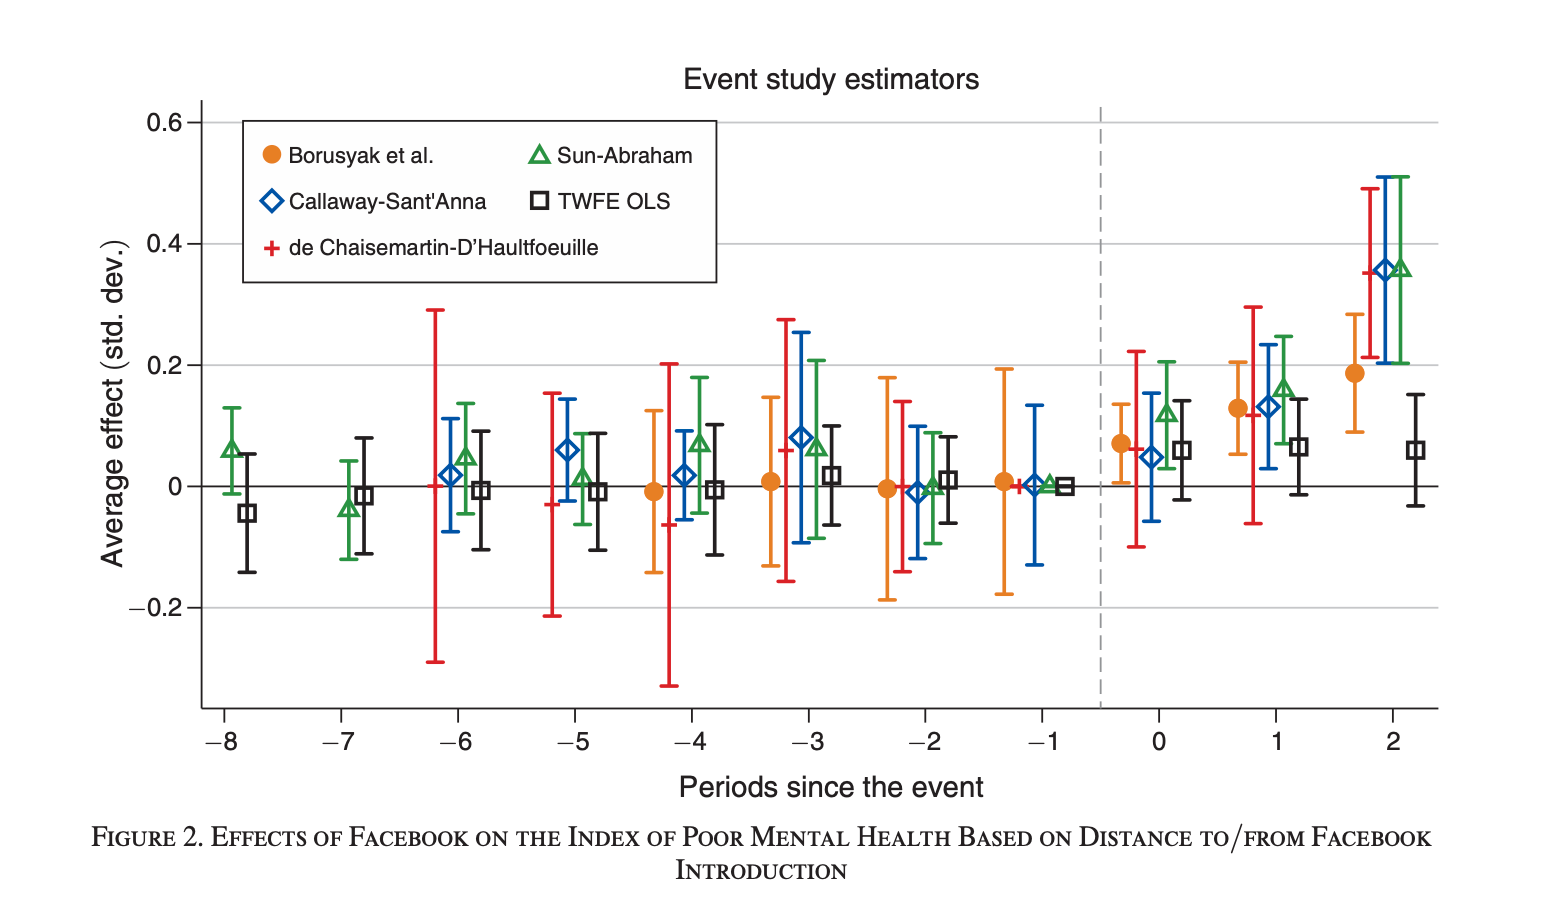
\includegraphics[height=4.1cm]{figs/remix10-13.png}
\end{center}
\src{Braghieri, Levy and Makarin (2022), Facebook's rollout and student mental health; Cunningham (2025), Figure 10.13.}

\begin{itemize}
\tightlist
\item
  Five estimators, one figure. Less reassuring than it looks: different
  controls, baselines, weights and assumptions. They are not robustness
  checks for one another.
\item
  Pick the estimator from the design, before the results. If you truly
  cannot choose in advance, report both.
\end{itemize}
\end{frame}

\begin{frame}{Honest DiD (Rambachan and Roth 2023)}
\protect\phantomsection\label{honest-did-rambachan-and-roth-2023}
\begin{itemize}
\tightlist
\item
  We already use pre-trends as \emph{evidence about} parallel trends,
  informally. Make it formal:

  \begin{itemize}
  \tightlist
  \item
    bound how badly parallel trends may fail \textbf{after} treatment,
    relative to before;
  \item
    report the set of ATTs consistent with the data under each bound.
  \end{itemize}
\item
  Two common bounds:

  \begin{itemize}
  \tightlist
  \item
    \textbf{relative magnitudes}: the post-period violation is at most
    \(M\) times the largest pre-period violation. \(M = 0\) is parallel
    trends; \(M = 1\) lets the post period go as wrong as the pre period
    ever did;
  \item
    \textbf{smoothness}: the differential trend may bend by at most
    \(M\) per period. \(M = 0\) extrapolates a linear pre-trend.
  \end{itemize}
\item
  The set widens with \(M\). The question is \textbf{at what \(M\) it
  first covers zero.}
\end{itemize}
\end{frame}

\begin{frame}{Honest DiD in practice: legal services and welfare}
\protect\phantomsection\label{honest-did-in-practice-legal-services-and-welfare}
\begin{center}
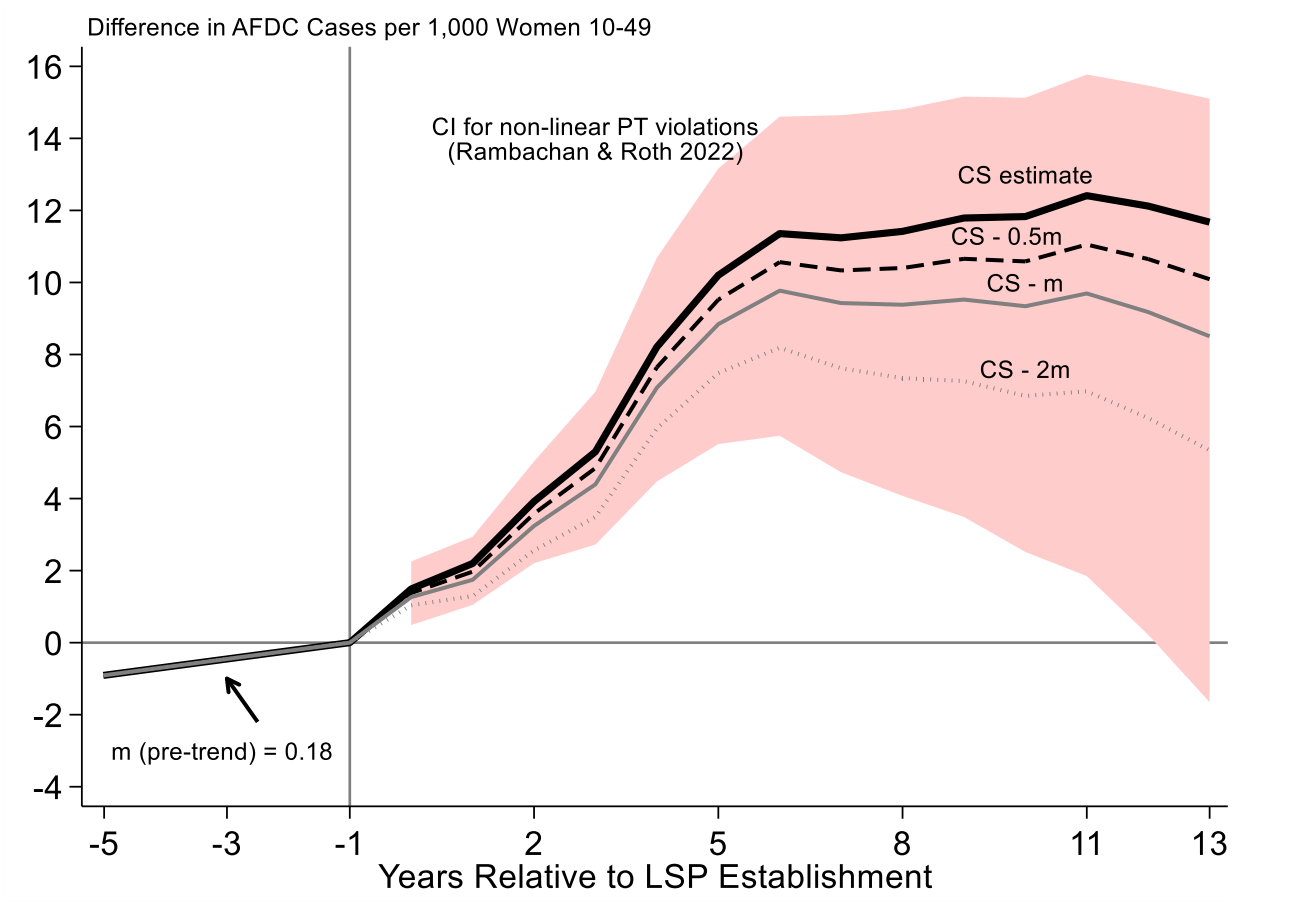
\includegraphics[height=4.4cm]{figs/remix10-14.png}
\end{center}
\src{Cunningham and Goodman-Bacon (2024), Figure 5; Cunningham (2025), Figure 10.14.}

\begin{itemize}
\tightlist
\item
  Pre-trend \(m \approx 0.2\) AFDC cases per \(1{,}000\) women a year.
  Netting out linear trends of \(0.1\)--\(0.4\) leaves long-run effects
  of \(7.5\)--\(10.5\).
\item
  Smoothness bound \(M = 0.1\) (shaded): zero is rejected at every event
  time but the last two.
\end{itemize}
\end{frame}

\begin{frame}[fragile]{What honest DiD is, and is not}
\protect\phantomsection\label{what-honest-did-is-and-is-not}
\begin{itemize}
\tightlist
\item
  \textbf{Not} a test that parallel trends failed. Parallel trends
  concerns counterfactuals and cannot be tested.
\item
  It states \textbf{how far parallel trends can fail before the
  conclusion does.}
\item
  A robustness check that \textbf{removes} an assumption instead of
  adding a model.
\item
  R and Stata: \texttt{honestdid}.
\end{itemize}
\end{frame}

\section{6. A Checklist}\label{a-checklist}

\begin{frame}{Ten steps, in order}
\protect\phantomsection\label{ten-steps-in-order}
\begin{enumerate}
\tightlist
\item
  \textbf{Define the target parameter}: which potential outcomes, which
  population, which weights.
\item
  \textbf{Count the units in each cohort}, including never- and
  always-treated.
\item
  \textbf{Plot the rollout.}
\item
  \textbf{Pick the control group} and defend it.
\item
  \textbf{Unconditional or conditional} parallel trends; if conditional,
  which covariates.
\item
  \textbf{Check imbalance}, several ways.
\item
  \textbf{Plot average outcomes by cohort}: the first time you look at
  \(Y\).
\item
  \textbf{Choose the estimator} from the design; state its assumptions.
\item
  \textbf{Falsify}: event study, placebos, sensitivity bounds. Know how
  your pre-trends were computed.
\item
  \textbf{DDDiD}, Don't Do Diff-in-Diff. Fold a losing hand early.
\end{enumerate}
\end{frame}

\begin{frame}{Why an order, and the running example}
\protect\phantomsection\label{why-an-order-and-the-running-example}
\begin{itemize}
\tightlist
\item
  Steps \(1\)--\(6\) never look at the outcome. Design before analysis
  (Rubin 2008).
\item
  Each step closes off a ``forking path'' before the results can tempt
  you down it.
\end{itemize}

\vspace{0.4em}

\begin{itemize}
\tightlist
\item
  \textbf{Running example:} Dias and Fontes (2024). Brazil's
  mental-health reform moved patients from psychiatric hospitals to
  community centres (CAPS).
\item
  CAPS opened in about \(1{,}600\) municipalities, \(2002\)--\(2016\).
  Outcome: homicide rate.
\item
  Question: did deinstitutionalization raise violence?
\end{itemize}
\end{frame}

\begin{frame}{Step 1: the parameter comes before the model}
\protect\phantomsection\label{step-1-the-parameter-comes-before-the-model}
Ten people in two municipalities, each with both potential outcomes for
``murdered'':

\begin{center}\small
\begin{tabular}{lcc}
\toprule
Municipality & Residents & Average $\delta_i$ \\
\midrule
1 (urban) & 8 & $0.50$ \\
2 (rural) & 2 & $-1.00$ \\
\midrule
ATE, average municipality: $\tfrac12(0.50 - 1.00)$ & & $-0.25$ \\
ATE, average person: $\tfrac{1}{10}(8 \times 0.50 - 2 \times 1.00)$ & & $0.20$ \\
\bottomrule
\end{tabular}
\end{center}

\begin{itemize}
\tightlist
\item
  Same ten effects, two correct averages, \textbf{opposite signs}.
\item
  Weighting municipal data by population recovers the per-person number;
  not weighting answers for the average municipality.
\end{itemize}
\end{frame}

\begin{frame}{Step 1: when the two averages diverge}
\protect\phantomsection\label{step-1-when-the-two-averages-diverge}
\begin{center}
\includegraphics[width=0.84\linewidth,height=\textheight,keepaspectratio]{07c_did_staggered_files/figure-beamer/texas-1.pdf}
\end{center}

\src{Simulated, after Cunningham (2025), Figure 10.16: the people with the largest effects live in the five big urban counties.}

\begin{itemize}
\tightlist
\item
  They diverge when effects are \textbf{heterogeneous} and people
  \textbf{sort} on them (Solon, Haider and Wooldridge 2015). Per person:
  \(2\). Per county: \(-0.88\).
\item
  Neither is biased. Choose by \textbf{who decides}: a mayor cares about
  the average municipality, a ministry about the average person.
\end{itemize}
\end{frame}

\begin{frame}[fragile]{Steps 2--3: count the cohorts, plot the rollout}
\protect\phantomsection\label{steps-23-count-the-cohorts-plot-the-rollout}
\begin{columns}[T]
\begin{column}{0.52\linewidth}
\begin{center}\small
\begin{tabular}{lcc}
\toprule
CAPS cohort & Munic. & Share \\
\midrule
2003 & 47 & 0.03 \\
2006 (largest) & 216 & 0.16 \\
2016 & 78 & 0.06 \\
Treated 2003--16 & 1,344 & 1.00 \\
Always-treated (2002) & 296 & -- \\
Never-treated & 3,836 & -- \\
\bottomrule
\end{tabular}
\end{center}
\end{column}

\begin{column}{0.48\linewidth}
\begin{center}
\adjincludegraphics[height=4.2cm, trim={{.04\width} {.25\height} {.03\width} {.22\height}}, clip]{figs/remix10-17.png}
\end{center}
\src{Cunningham (2025), Figure 10.17.}
\end{column}
\end{columns}

\begin{itemize}
\tightlist
\item
  \textbf{Always-treated} units have no untreated baseline: drop them.
\item
  The largest cohort will dominate any aggregation. Know that before you
  aggregate.
\item
  The rollout plot (\texttt{panelView} in R and Stata) shows the
  not-yet-treated pool shrinking year by year.
\end{itemize}
\end{frame}

\begin{frame}{Step 4: choose the control group}
\protect\phantomsection\label{step-4-choose-the-control-group}
\begin{itemize}
\tightlist
\item
  The more random the assignment, the less the choice matters.
\item
  CAPS placement was not random. The never-treated municipalities are
  small and rural.
\item
  Not-yet-treated municipalities, which did get a CAPS eventually, may
  be the closer comparison.
\item
  Decide \textbf{before} results. Unsure? Run both and report both.
\end{itemize}
\end{frame}

\begin{frame}{Steps 5--6: covariates and balance}
\protect\phantomsection\label{steps-56-covariates-and-balance}
\begin{itemize}
\tightlist
\item
  Conditional parallel trends needs covariates that drive \textbf{both}
  CAPS placement and homicide trends: economics, demographics,
  urbanization, policing, social programmes.
\item
  Cunningham uses Dias and Fontes's list rather than his own: a
  specification chosen by someone who had not seen these results.
\item
  Standardized differences at baseline, treated vs.~never-treated:

  \begin{itemize}
  \tightlist
  \item
    rural share \(-0.60\); population \(0.69\);
  \item
    health spending \(-0.45\); women aged 20--29 \(0.75\).
  \end{itemize}
\item
  Many are past \(0.25\). Those go in.
\end{itemize}
\end{frame}

\begin{frame}[fragile]{Step 6: look at the propensity score}
\protect\phantomsection\label{step-6-look-at-the-propensity-score}
\begin{columns}[T]
\begin{column}{0.55\linewidth}
\begin{center}
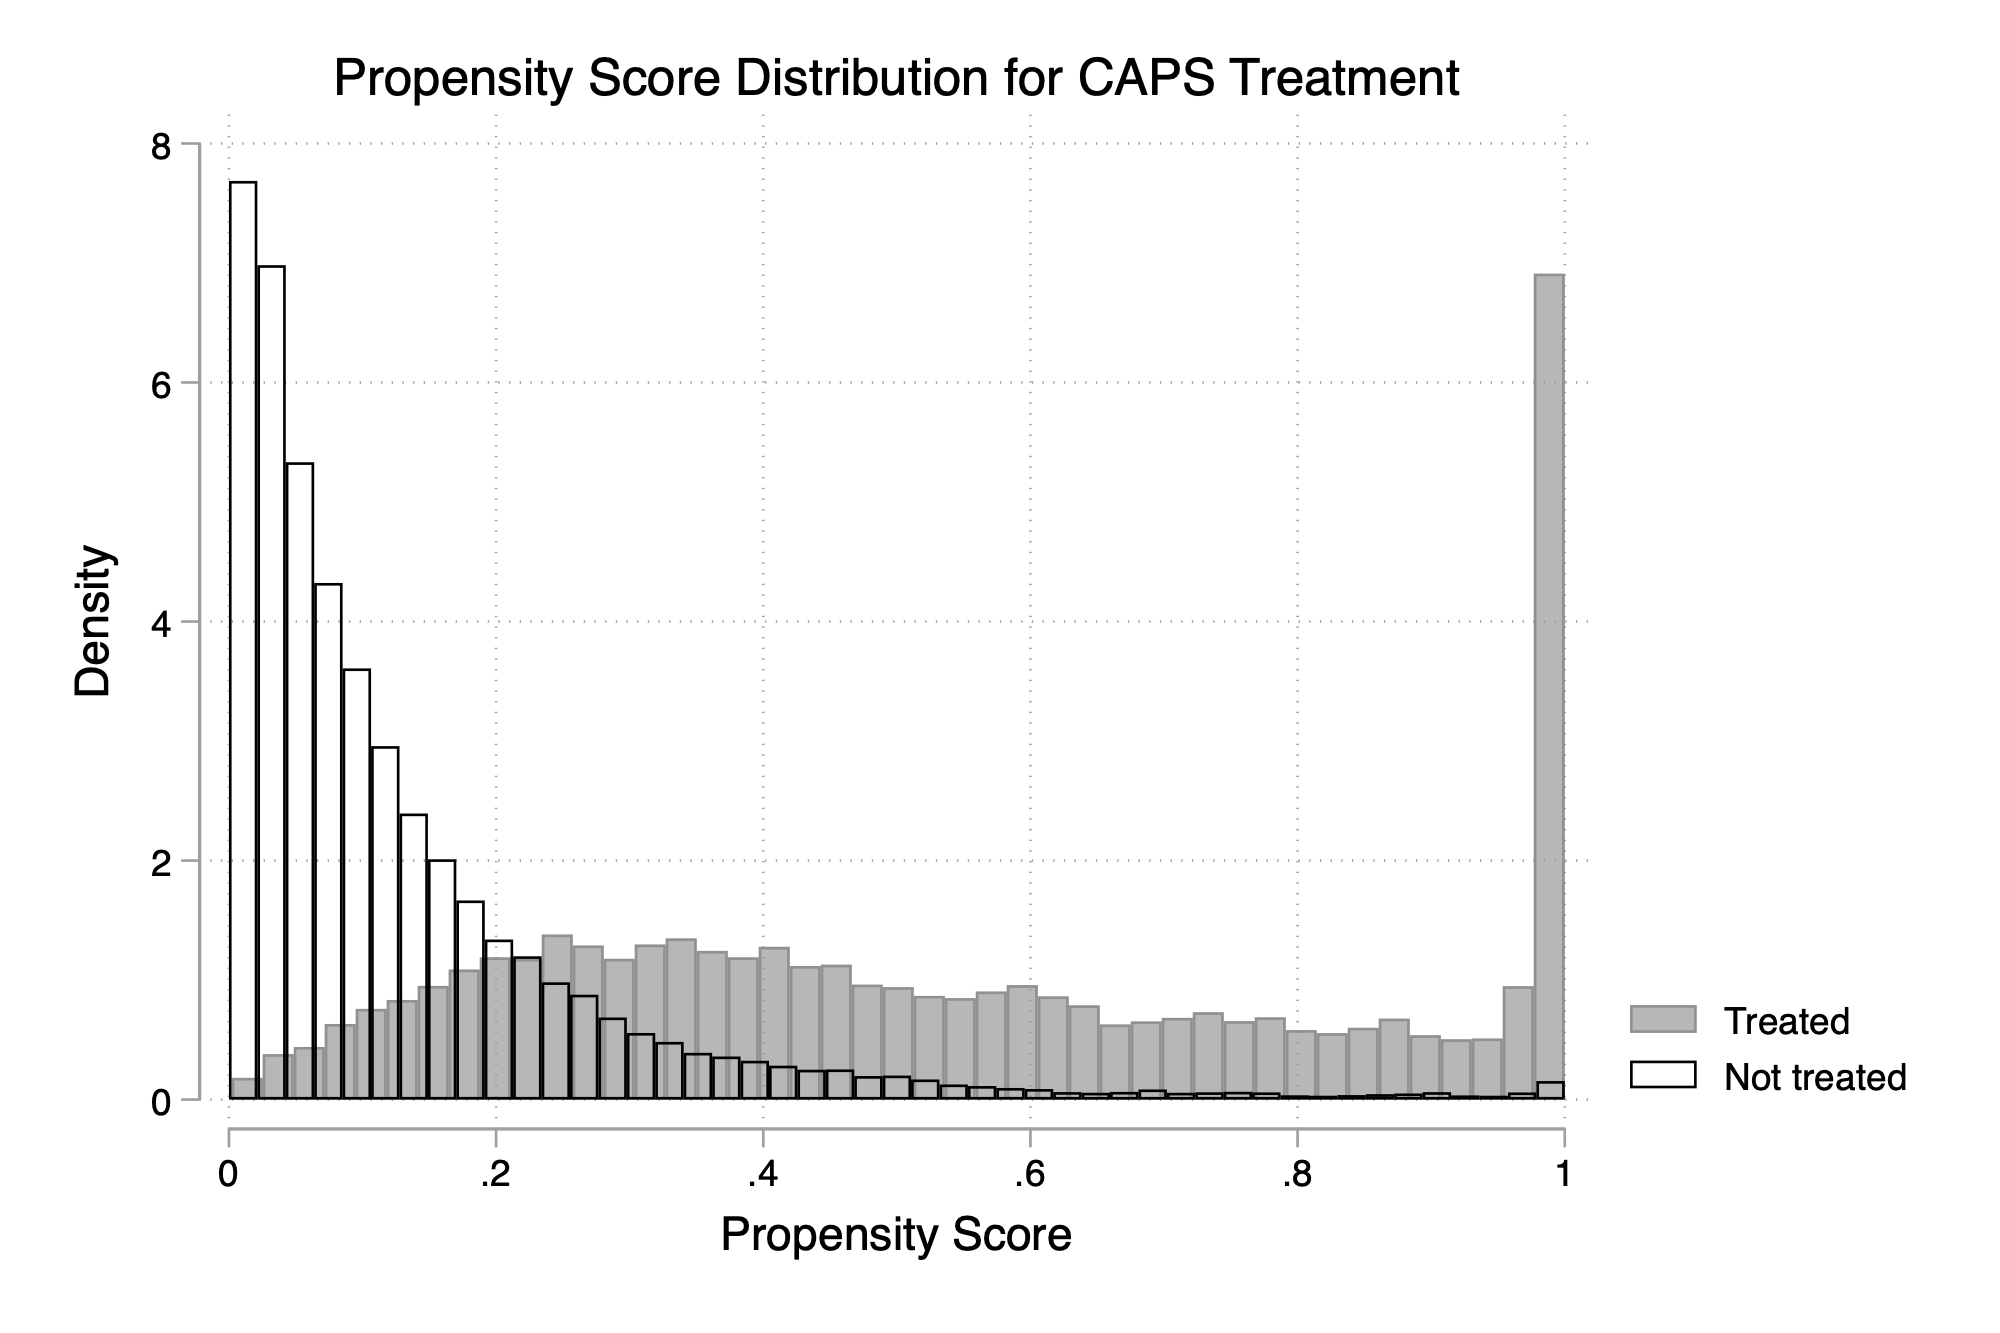
\includegraphics[height=4.3cm]{figs/remix10-19.png}
\end{center}
\src{Cunningham (2025), Figure 10.19.}
\end{column}

\begin{column}{0.45\linewidth}
\small

\begin{itemize}
\tightlist
\item
  Controls pile up near zero; a spike of treated near one.
\item
  \(11\) control municipalities above \(0.995\). One at \(0.999971\)
  gets weight \[
  \frac{0.999971}{1 - 0.999971} \approx 34{,}000 .
  \]
\item
  One municipality counts as thirty-four thousand. Trim before
  estimating.
\item
  R's \texttt{did} trims automatically; not every package does.
\end{itemize}
\end{column}
\end{columns}
\end{frame}

\begin{frame}[fragile]{Steps 7--8: look at the outcome, then estimate}
\protect\phantomsection\label{steps-78-look-at-the-outcome-then-estimate}
\begin{itemize}
\tightlist
\item
  \textbf{Step 7.} Mean homicide rate by cohort over time: trends
  similar, \textbf{levels} very different, never-treated lowest of all.

  \begin{itemize}
  \tightlist
  \item
    That is the rural pattern from the balance table: \(76\) percent of
    Brazil's homicides are urban.
  \item
    Kahn-Lang and Lang again: explain the levels.
  \end{itemize}
\item
  \textbf{Step 8.} Callaway--Sant'Anna, doubly robust, not-yet-treated
  controls, long differences, with the imbalanced covariates:
\end{itemize}

\vspace{0.2em}
\scriptsize

\texttt{csdid2\ homicide\_rate\ \$controls,\ gvar(g)\ ivar(cod)\ time(ano)\ long2\ method(drimp)\ notyet}
\normalsize
\end{frame}

\begin{frame}{Step 8: the results}
\protect\phantomsection\label{step-8-the-results}
\begin{columns}[T]
\begin{column}{0.5\linewidth}
\begin{center}
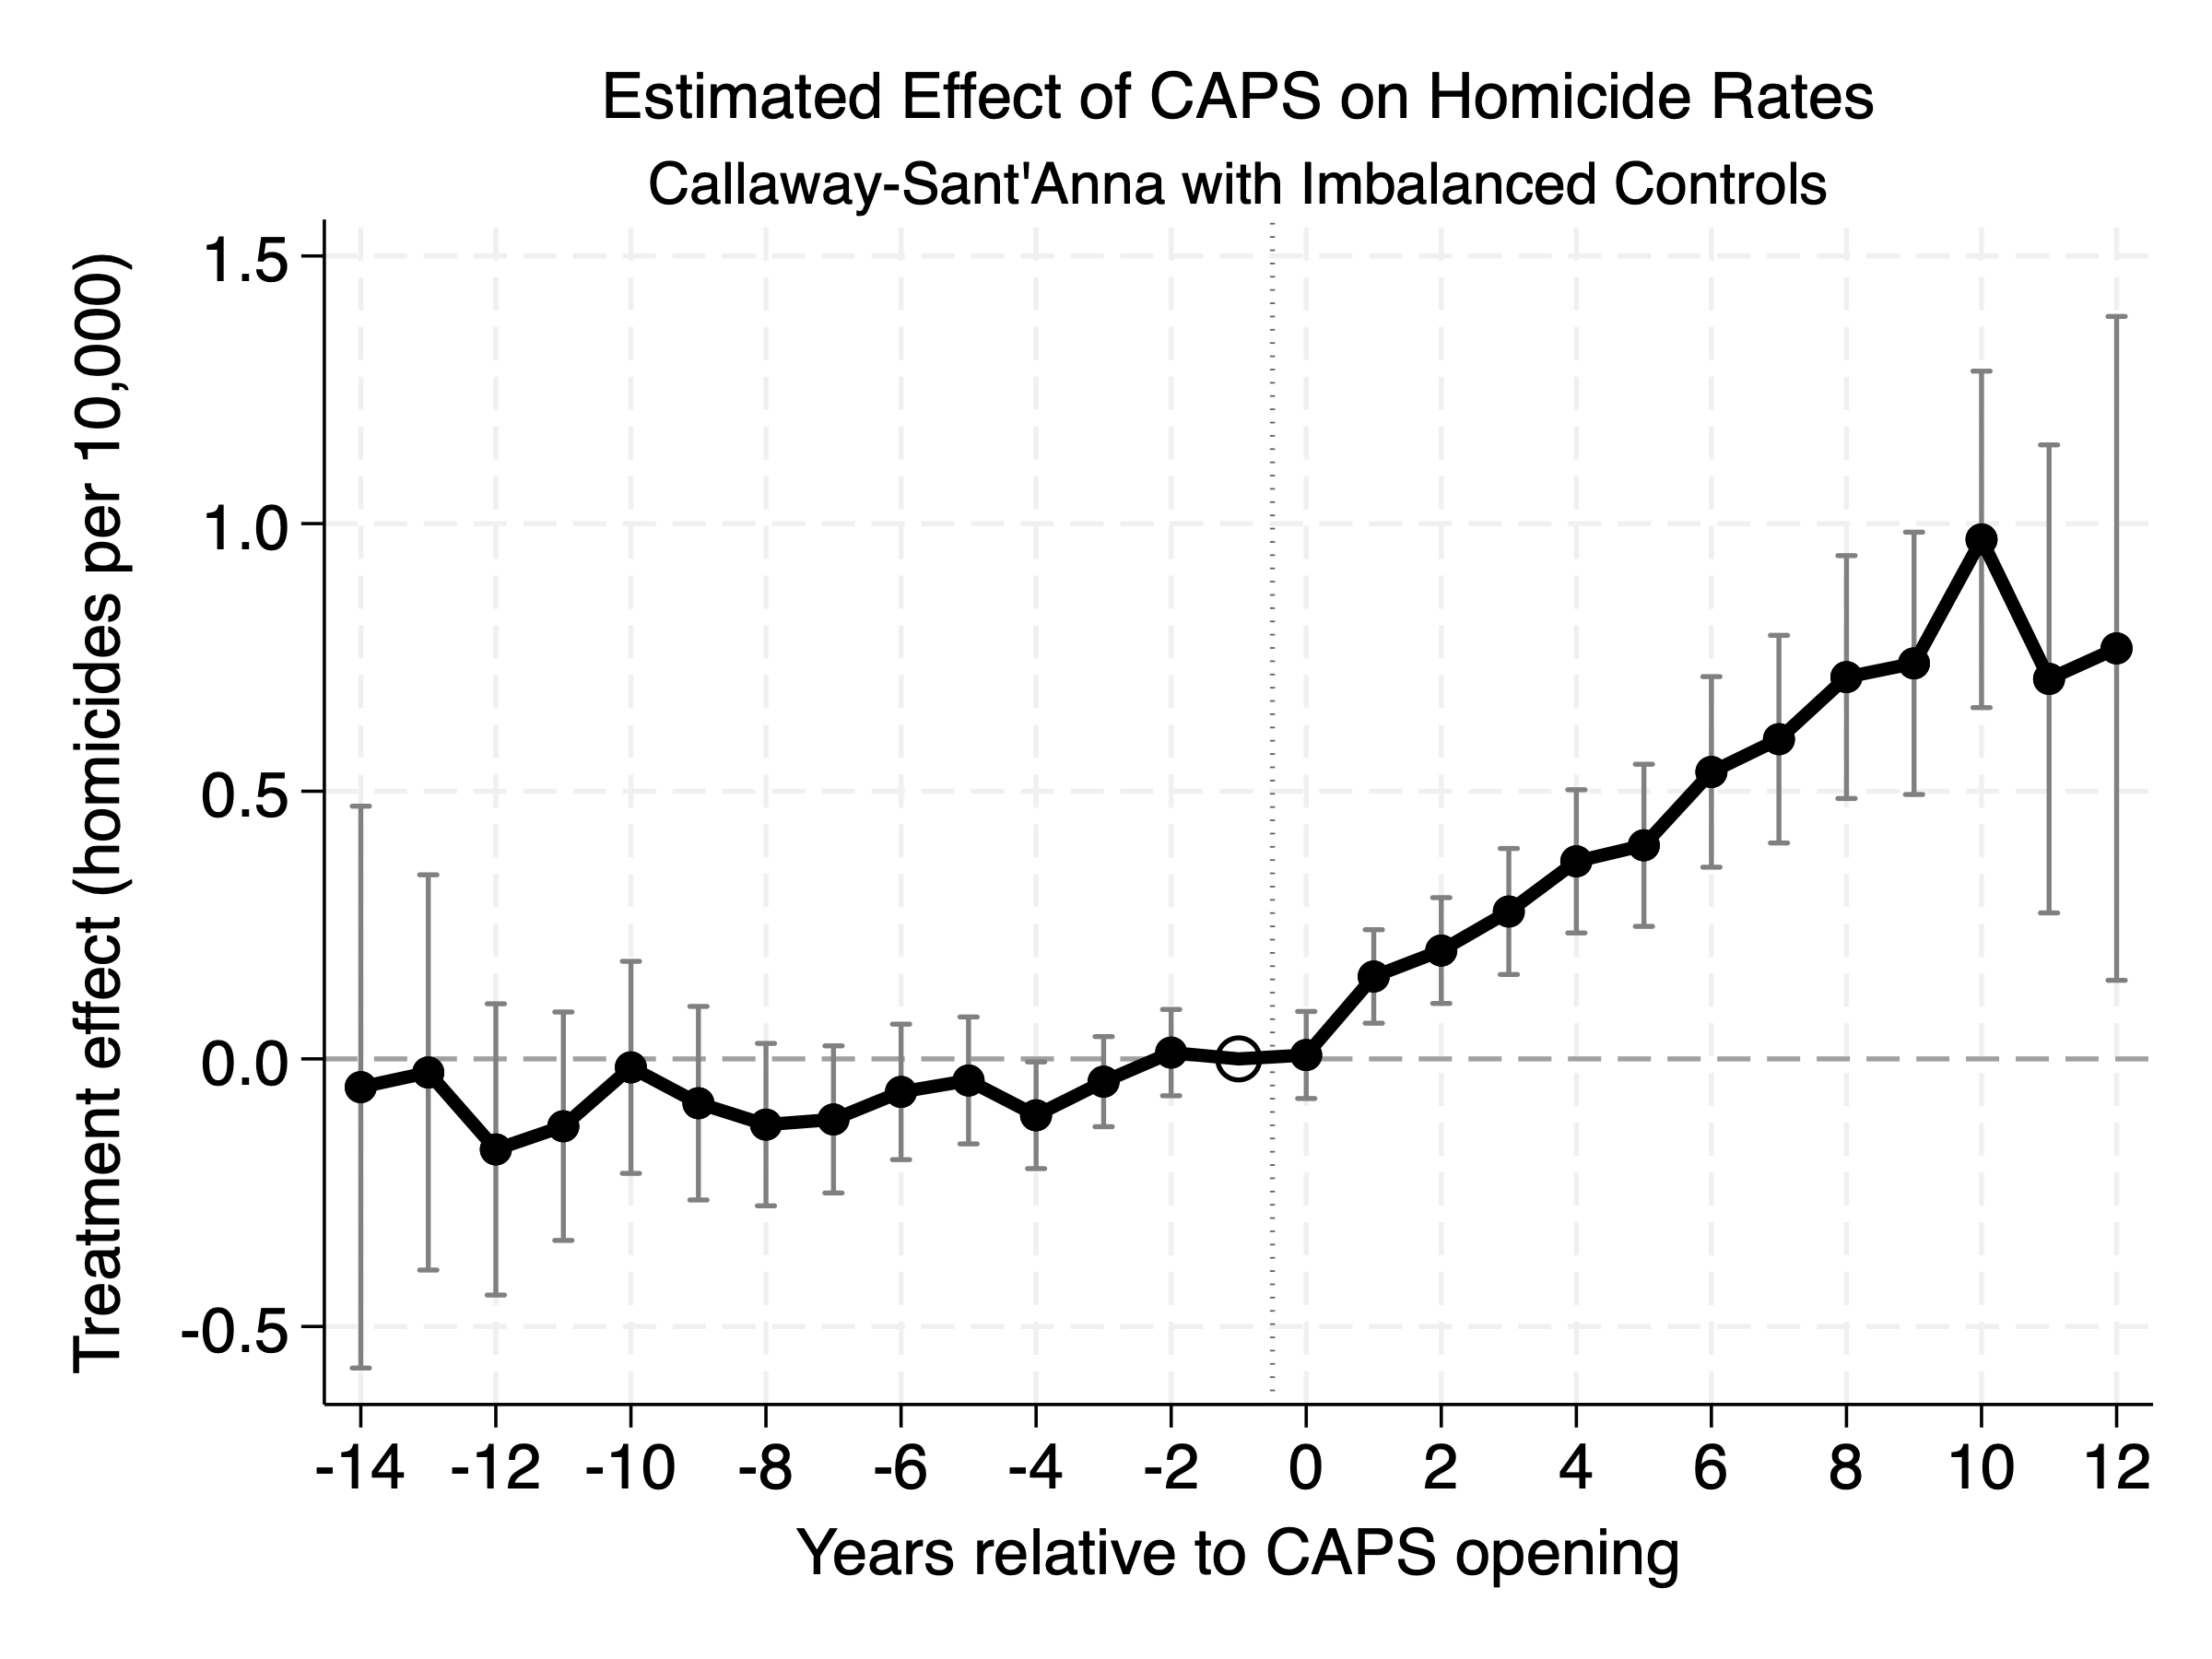
\includegraphics[height=3.9cm]{figs/remix10-22.png}

\footnotesize All leads and lags
\end{center}
\end{column}

\begin{column}{0.5\linewidth}
\begin{center}
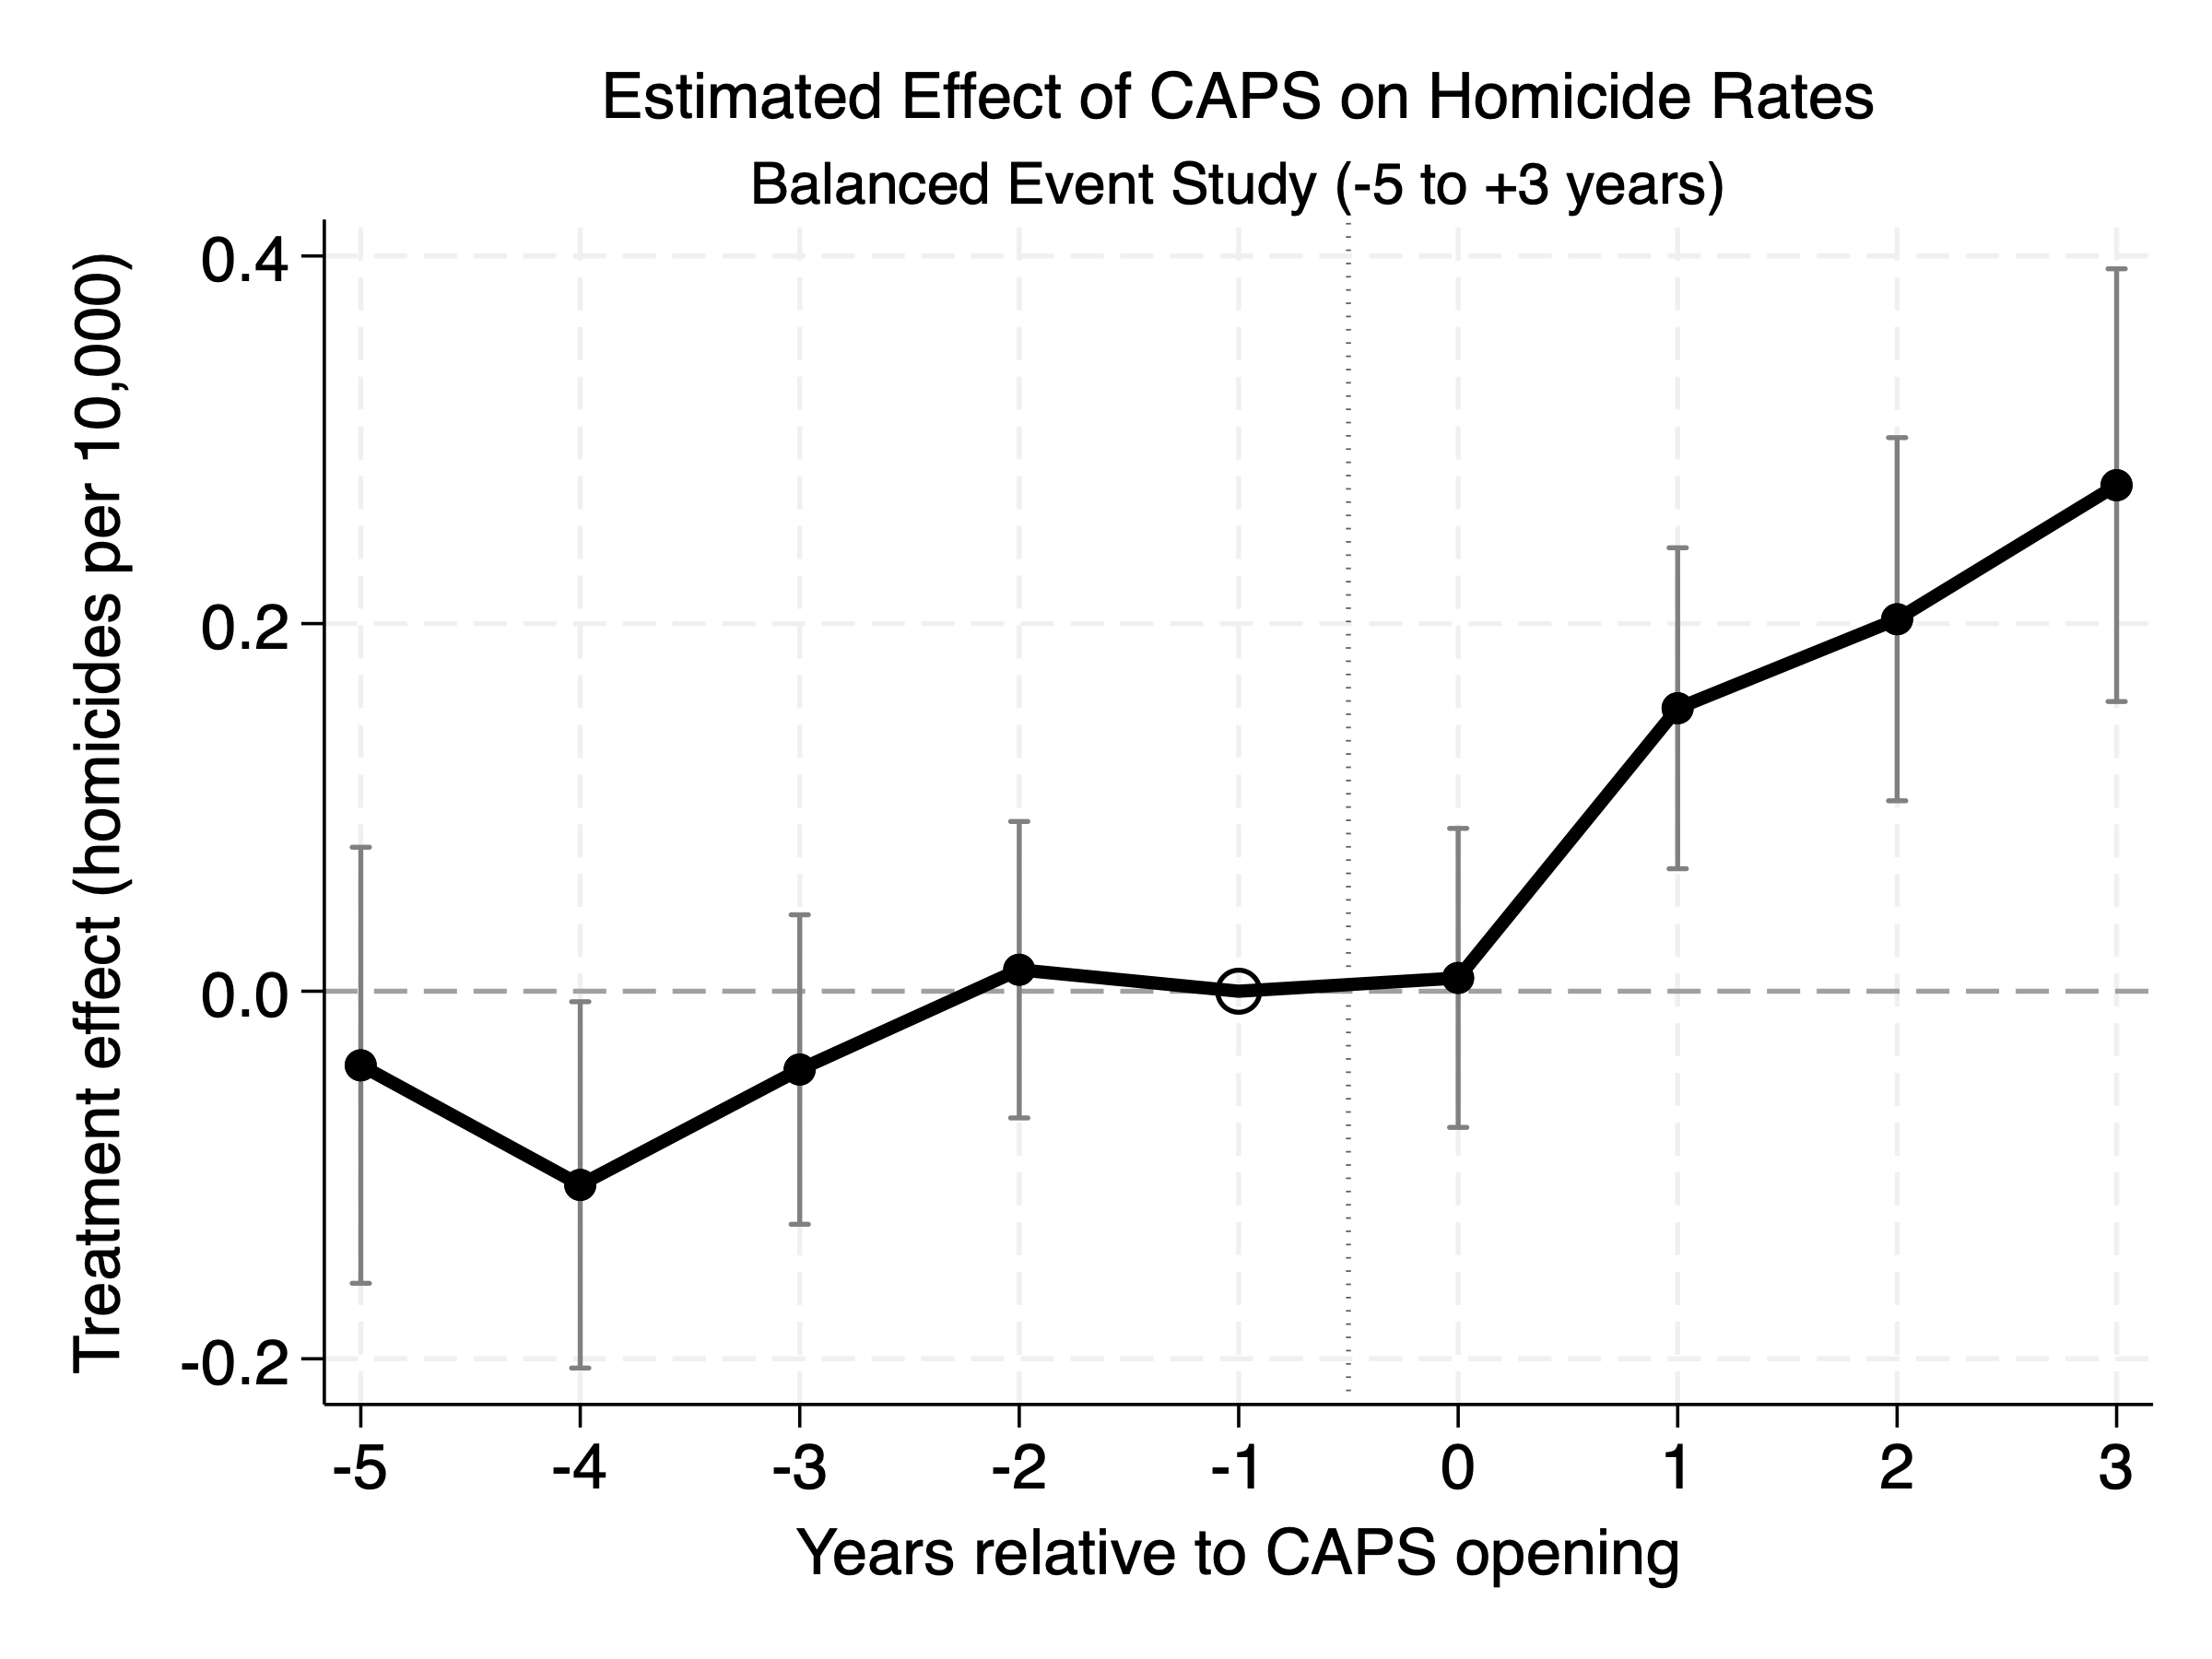
\includegraphics[height=3.9cm]{figs/remix10-23.png}

\footnotesize Balanced window, $-5$ to $+3$
\end{center}
\end{column}
\end{columns}

\src{Cunningham (2025), Figures 10.22 and 10.23.}

\begin{itemize}
\tightlist
\item
  \textbf{All:} pre-period average \(-0.073\) (\(0.069\)); post average
  \(0.495\) (\(0.080\)), about \(1\) homicide per \(10{,}000\) after ten
  years.
\item
  But the far right is \textbf{three early cohorts} and the far left is
  late adopters: the composition changes along the axis.
\end{itemize}
\end{frame}

\begin{frame}{Step 8: why restrict the window}
\protect\phantomsection\label{step-8-why-restrict-the-window}
\begin{itemize}
\tightlist
\item
  In the full plot, each point averages a \textbf{different set of
  cohorts}. A rising line may be rising effects, or a change in who is
  averaged.
\item
  In a window where most cohorts contribute, \(-5\) to \(+3\), the
  composition is roughly fixed.
\item
  There: effects positive from the first full year, about \(0.275\) per
  \(10{,}000\) at \(\ell = +3\) against a baseline of \(1.38\), roughly
  \(20\) percent.
\item
  The lead at \(\ell = -4\) is negative and significant: something for
  step 9.
\end{itemize}
\end{frame}

\begin{frame}{Step 9: how wrong can parallel trends be?}
\protect\phantomsection\label{step-9-how-wrong-can-parallel-trends-be}
\begin{columns}[T]
\begin{column}{0.52\linewidth}
\begin{center}
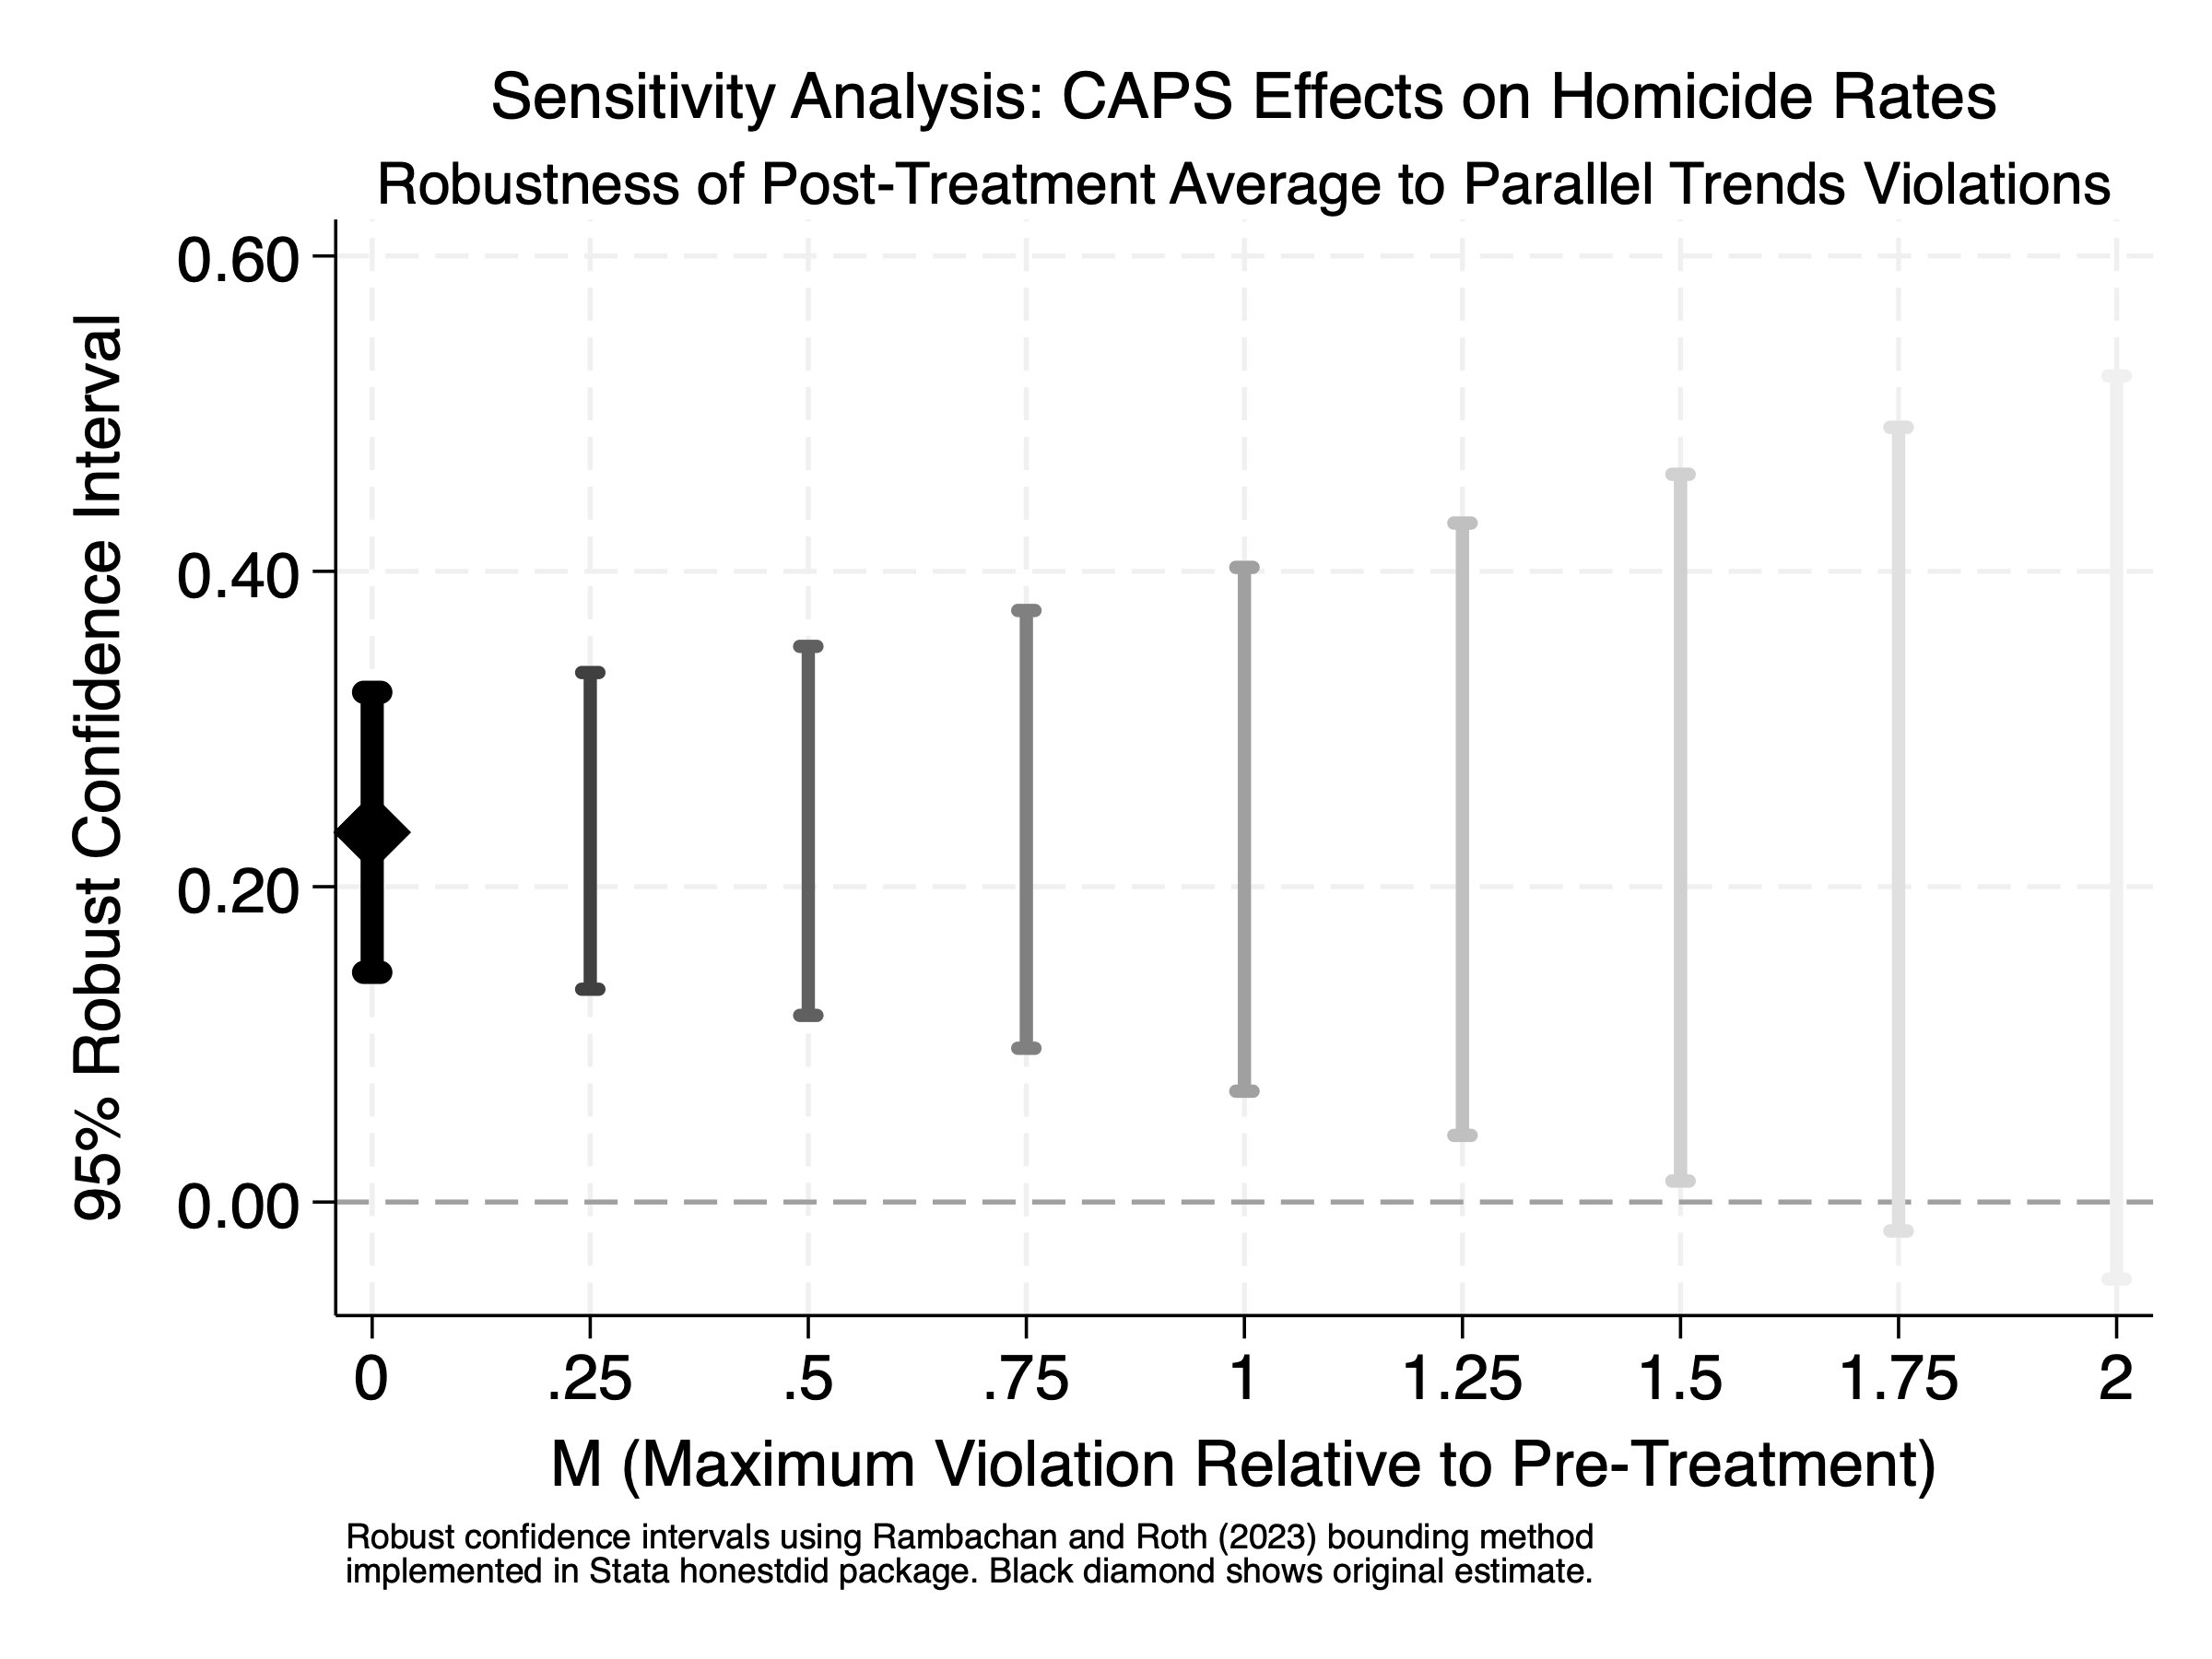
\includegraphics[height=4.4cm]{figs/remix10-24.png}
\end{center}
\src{Cunningham (2025), Figure 10.24.}
\end{column}

\begin{column}{0.48\linewidth}
\small

\begin{itemize}
\tightlist
\item
  Honest DiD on the average of the four post lags, \(0.234\).
\item
  Relative magnitudes: the set excludes zero up to \(M = 1.5\),
  post-period violations one and a half times the worst pre-period
  violation.
\item
  The result survives.
\item
  Cunningham was sceptical and now is not: a different estimator, a
  checklist and tolerant bounds all agree.
\end{itemize}
\end{column}
\end{columns}
\end{frame}

\begin{frame}{Step 10: when to walk away}
\protect\phantomsection\label{step-10-when-to-walk-away}
\begin{itemize}
\tightlist
\item
  Every estimator in these two lectures rests on parallel trends.
\item
  Put the design down when you cannot believe it with a straight face:

  \begin{itemize}
  \tightlist
  \item
    the selection mechanism in Ghanem, Sant'Anna and Wüthrich (2024) is
    clearly at work;
  \item
    common support is unattainable;
  \item
    the pre-trends are a roller coaster;
  \item
    the bounds collapse at \(M = 0.2\).
  \end{itemize}
\item
  Imbens's ``DDDiD'': Don't Do Diff-in-Diff.
\item
  Next lecture: one of the alternatives, synthetic control.
\end{itemize}
\end{frame}

\begin{frame}{Conclusion}
\protect\phantomsection\label{conclusion}
\begin{enumerate}
\tightlist
\item
  \textbf{Build, then aggregate.} CS estimates each \(\text{ATT}(g,t)\)
  as a clean \(2 \times 2\) and averages with weights you choose.
\item
  \textbf{Honest estimators may target less.} Cells without an untreated
  comparison are not identified by anyone; say what you estimate.
\item
  \textbf{TWFE event studies are contaminated} when cohorts have
  different effect paths, or when software drops periods. Sun--Abraham's
  interaction weights fix it.
\item
  \textbf{dCDH} handles treatments that switch off; \textbf{imputation}
  buys efficiency with stronger parallel trends. Choose by the
  assumption.
\item
  \textbf{Read event studies carefully}: long differences vs.~short
  gaps, the imputation kink, honest bounds instead of ``the pre-trends
  look fine.''
\item
  \textbf{Checklist.} Parameter, cohorts, rollout, controls, covariates,
  balance; then the outcome, the estimator, the bounds. If it is not
  credible, walk away.
\end{enumerate}
\end{frame}

\begin{frame}{References}
\protect\phantomsection\label{references}
\tiny

\begin{itemize}
\tightlist
\item
  Baker, A. C., D. F. Larcker and C. C. Y. Wang (2022). How Much Should
  We Trust Staggered Difference-in-Differences Estimates? \emph{Journal
  of Financial Economics} 144(2), 370--395.
\item
  Baker, A., B. Callaway, S. Cunningham, A. Goodman-Bacon and P.
  Sant'Anna (2025). Difference-in-Differences Designs: A Practitioner's
  Guide. Working paper.
\item
  Borusyak, K., X. Jaravel and J. Spiess (2024). Revisiting Event-Study
  Designs: Robust and Efficient Estimation. \emph{Review of Economic
  Studies} 91(6), 3253--3285.
\item
  Braghieri, L., R. Levy and A. Makarin (2022). Social Media and Mental
  Health. \emph{AER} 112(11), 3660--3693.
\item
  Callaway, B. and P. Sant'Anna (2021). Difference-in-Differences with
  Multiple Time Periods. \emph{Journal of Econometrics} 225(2),
  200--230.
\item
  de Chaisemartin, C. and X. D'Haultfoeuille (2020). Two-Way Fixed
  Effects Estimators with Heterogeneous Treatment Effects. \emph{AER}
  110(9), 2964--2996.
\item
  Cheng, C. and M. Hoekstra (2013). Does Strengthening Self-Defense Law
  Deter Crime or Escalate Violence? Evidence from Expansions to Castle
  Doctrine. \emph{Journal of Human Resources} 48(3), 821--854.
\item
  Cunningham, S. (2025). \emph{Causal Inference: The Remix}, ch.~10 ---
  the source for this lecture, including the Baker simulation data and
  the reproduced figures.
\item
  Cunningham, J. and A. Goodman-Bacon (2024). Legal Services, Divorce
  and Welfare. Working paper.
\item
  Dias, M. and L. F. Fontes (2024). The Effects of a Large-Scale Mental
  Health Reform: Evidence from Brazil. Working paper.
\item
  Gardner, J. (2021). Two-Stage Differences-in-Differences. Working
  paper.
\item
  Ghanem, D., P. Sant'Anna and K. Wüthrich (2024). Selection and
  Parallel Trends. Working paper.
\item
  Goldsmith-Pinkham, P., P. Hull and M. Kolesár (2024). Contamination
  Bias in Linear Regressions. \emph{AER} 114(12), 4015--4051.
\end{itemize}
\end{frame}

\begin{frame}{References (cont.)}
\protect\phantomsection\label{references-cont.}
\tiny

\begin{itemize}
\tightlist
\item
  Goodman-Bacon, A. (2021). Difference-in-Differences with Variation in
  Treatment Timing. \emph{Journal of Econometrics} 225(2), 254--277.
\item
  Kahn-Lang, A. and K. Lang (2020). The Promise and Pitfalls of
  Differences-in-Differences: Reflections on 16 and Pregnant and Other
  Applications. \emph{JBES} 38(3), 613--620.
\item
  Rambachan, A. and J. Roth (2023). A More Credible Approach to Parallel
  Trends. \emph{Review of Economic Studies} 90(5), 2555--2591.
\item
  Roth, J. (2024). Interpreting Event-Studies from Recent
  Difference-in-Differences Methods. Working paper.
\item
  Rubin, D. B. (2008). For Objective Causal Inference, Design Trumps
  Analysis. \emph{Annals of Applied Statistics} 2(3), 808--840.
\item
  Solon, G., S. Haider and J. Wooldridge (2015). What Are We Weighting
  For? \emph{Journal of Human Resources} 50(2), 301--316.
\item
  Sun, L. and S. Abraham (2021). Estimating Dynamic Treatment Effects in
  Event Studies with Heterogeneous Treatment Effects. \emph{Journal of
  Econometrics} 225(2), 175--199.
\item
  Wooldridge, J. M. (2021). Two-Way Fixed Effects, the Two-Way Mundlak
  Regression, and Difference-in-Differences Estimators. Working paper.
\end{itemize}
\end{frame}

\section{Backup}\label{backup}

\begin{frame}[fragile]{Stata: the estimators of this lecture}
\protect\phantomsection\label{stata-the-estimators-of-this-lecture}
\begin{Shaded}
\begin{Highlighting}[]
\KeywordTok{use}\NormalTok{ https:}\CommentTok{//raw.githubusercontent.com/scunning1975/mixtape/master/baker.dta, clear}
\NormalTok{csdid2 }\FunctionTok{y}\NormalTok{, ivar(id) time(}\FunctionTok{year}\NormalTok{) gvar(treat\_date) notyet method(stdipw) long2}
\KeywordTok{estat}\NormalTok{ simple                                         }\CommentTok{// 68.3}
\KeywordTok{estat} \FunctionTok{group}                                          \CommentTok{// 56}
\KeywordTok{estat}\NormalTok{ event                                          }\CommentTok{// relative{-}time aggregation}
\NormalTok{eventstudyinteract }\FunctionTok{y}\NormalTok{ lead* lag*, cohort(treat\_date) control\_cohort(}\FunctionTok{last}\NormalTok{) absorb(id }\FunctionTok{year}\NormalTok{)}
\NormalTok{did\_imputation }\FunctionTok{y}\NormalTok{ id }\FunctionTok{year}\NormalTok{ treat\_date, autosample      }\CommentTok{// Borusyak{-}Jaravel{-}Spiess}
\NormalTok{did\_multiplegt\_dyn }\FunctionTok{y}\NormalTok{ id }\FunctionTok{year}\NormalTok{ treat                   }\CommentTok{// de Chaisemartin{-}D\textquotesingle{}Haultfoeuille}
\NormalTok{twowayfeweights }\FunctionTok{y}\NormalTok{ id }\FunctionTok{year}\NormalTok{ treat, }\DecValTok{type}\NormalTok{(feTR)          }\CommentTok{// share of negative TWFE weights}
\NormalTok{honestdid, pre(1/4) }\KeywordTok{post}\NormalTok{(5/8) mvec(0(0.5)2)          }\CommentTok{// Rambachan{-}Roth, after an event study}
\end{Highlighting}
\end{Shaded}

\begin{itemize}
\tightlist
\item
  R equivalents: \texttt{did} (\texttt{att\_gt}, \texttt{aggte}),
  \texttt{fixest::sunab}, \texttt{didimputation},
  \texttt{DIDmultiplegtDYN}, \texttt{TwoWayFEWeights},
  \texttt{HonestDiD}. This deck computes CS and the imputation estimator
  from group means with \texttt{fixest} and base R only.
\end{itemize}
\end{frame}




\end{document}
